\documentclass[a4paper 12pt]{article}
\usepackage[margin=1in]{geometry}
\usepackage{natbib}
\usepackage{epsfig}
\usepackage{amsmath}
\usepackage{amsfonts}
\usepackage{float}
\usepackage{rotating} 
\usepackage{caption}
\usepackage{subfig}
\usepackage{booktabs}
\usepackage{adjustbox}
\usepackage[table]{xcolor}
\usepackage{tabularx}
\usepackage{caption}
\usepackage{enumerate}
\usepackage{enumitem}
\captionsetup{font=footnotesize}
\newcommand{\ra}[1]{\renewcommand{\arraystretch}{#1}}
\textheight 9.0 in
\textwidth 6.5 in
\topmargin -0.5 in
\oddsidemargin 0.0in
\renewcommand{\topfraction}{1}
\renewcommand{\bottomfraction}{1}
\renewcommand{\textfraction}{0}
\renewcommand{\floatpagefraction}{0.90}
\definecolor{TableEven}{rgb}{0.8000,0.9216,0.9490}
\usepackage{makecell}
%\usepackage{fourier} 
\numberwithin{equation}{section}
\usepackage{array}
\usepackage{titlesec}
\usepackage{sectsty}
\sectionfont{\centering}
\setcounter{secnumdepth}{4}
\usepackage{natbib}
\usepackage{siunitx}
\usepackage[toc,page]{appendix}
\usepackage{sectsty}
\usepackage{scalerel,stackengine}
\stackMath
\usepackage{graphicx}
%\titleformat{\subsection}    
%       {\normalfont\fontfamily{phv}\fontsize{12}{17}\bfseries\itshape}{\thesubsection}{1em}{}
\subsectionfont{\normalfont\bfseries\itshape}
\subsubsectionfont{\normalfont\itshape}
%\usepackage[colorlinks,citecolor=DeepPink4,linkcolor=DarkRed, urlcolor=DarkBlue]{hyperref}
%\usepackage[svgnames]{xcolor} 
%
%\usepackage[colorlinks]{hyperref}
%\hypersetup{citecolor=DeepPink4}
%\hypersetup{linkcolor=DarkRed}
%\hypersetup{urlcolor=DarkBlue}
%\usepackage{cleveref}

%hyperlink for website will need a better option. highlights all equations etc
 \usepackage{hyperref}


\renewcommand{\baselinestretch} {2.0}
\makeatletter
\setcounter{page}{1}
\def\doublespace{\def\baselinestretch{1}\@normalsize}
\def\enddoublespace{}
\title{\bf 
}   
% \footnotemark}
\author{}
\date{}
\@addtoreset{equation}{section}
\renewcommand{\sp}{\vspace{0.2 in}}
\renewcommand{\theequation} {\arabic{section}.\arabic{equation}}
%\renewcommand{\thefigure}{\arabic{section}.\arabic{figure}}
\renewcommand{\thefootnote}{\fnsymbol{footnote}}
\newtheorem{theorem}{Theorem}
\newtheorem{lemma}{Lemma}[section]
\newtheorem{remark}{Remark}[section]
\newtheorem{corollary}{Corollary}[section]
\newtheorem{exam}{Example}[section]
\newtheorem{proposition}{Proposition}[section]

\newcommand{\Bigskip}{\vspace{0.3 in}}

\usepackage{xspace}
\newcommand{\m}{\textnormal{\sffamily m}\xspace}
\newcommand{\cm}{\textnormal{\sffamily cm}\xspace}
\newcommand{\g}{\textnormal{\sffamily g}\xspace}
\newcommand{\kg}{\textnormal{\sffamily kg}\xspace}
\newcommand{\SE}{\textnormal{\sffamily SE}\xspace}
\newcommand{\RSE}{\textnormal{\sffamily RSE}\xspace}
\newcommand{\LB}{\textnormal{\sffamily LB}\xspace}
\newcommand{\UB}{\textnormal{\sffamily UB}\xspace}


\makeatletter
\let\latex@xfloat=\@xfloat
\def\@xfloat #1[#2]{%
  \latex@xfloat #1[#2]%
  \def\baselinestretch{1}
  \@normalsize\normalsize
  \normalsize
}
\makeatother

\newcommand\longitude[1]{\directlua{ longitude ( \luastring{#1} ) }}


\usepackage{lineno}
\linenumbers

 
\begin{document}
\title{Optimising sampling effort of the North Sea International Bottom Trawl Survey Data}

\maketitle


\begin{abstract}

In this research we present nonparametric estimation procedures for calculating abundance at age indices, and investigate the sensitivity of these estimates with respect to the number of otholits collected at sea. The procedures presented are applied to the North Sea International Bottom Trawls Survey data for cod (\textit{Gadus morhua}) and saithe (\textit{Pollachius virens}). We demonstrate how much information would be lost if the survey design was defined such that fewer otholits were collected. Age length keys (ALKs) are used to map lengths to age, and we use ALKs with and without the assumption of constant age length structures over relatively large areas. All abundance at age indices are presented with variance estimates. \\
%In this research we present an approach for optimising sampling effort of the North Sea International Bottom Trawl Survey Data. 

\end{abstract}


\section{Introduction}
Fish stock assessments are used by fishery managers for making management decisions regarding catch quotas. The assessments provide fundamental information about the status of the stock, for instance, whether the stock is increasing and support for increased levels of harvest should be given, or whether the stock is decreasing and stricter control on harvest should be implemented. Associated with the parameters used in fish stock assessment is their uncertainty, which should not be ignored when formulating management policies \citep{walters1981effects, ludwig1981measurement, berg2014evaluation}. This uncertainty can arise from many sources including natural variability, estimation procedures and lack of knowledge regarding the parameter \citep{ehrhardt1997role}. The North Sea International Bottom Trawl Survey (IBTS) data, coordinated by the International Council for the Exploration of the Sea (ICES), provides information on seasonal distribution of stocks and estimates of abundance indices and catch in numbers of fish per age-class without an assessment of the accuracy of these estimates. As stated by \citet{ludwig1981measurement} it is relevant for managers to take into the uncertainty related to stock size when making management polices. The indices of abundance at age from IBTS  are based on data obtained from a stratified semi-random sampling approach of trawl stations,  and  it is essential to account for the sampling approach so as to produce reliable variance estimates \citep{lehtonen2004practical}. If the sampling approach is ignored, the effect on the variance  of the parameters could be substantial.  In particular, the variance could be greatly inflated  due to the clustering effect, which involves intra-cluster correlation of the variables \citep{aanes2015efficient, lehtonen2004practical}. 

There are two separate stages for generating abundance indices per age from the North Sea International Bottom Trawl Survey (IBTS) data.  The first consist of calculating indices per \textit{length} class, which are obtained by trawling in a stratified manner and counting the number of fish caught. Then that knowledge is transformed to indices with respect to age. The latter part is achieved with an age-length key (ALK), which is constructed by sampling otoliths in a stratified procedure from each haul and/or sub-area. To our best knowledge, there has been no research on how much the uncertainty of the abundance indices is related to these two distinct parts. The main contribution of this research is to shed light on how the indices estimates and their associated uncertainty estimates change if less effort was spent on collection of otoliths. We achieve the reduction of otoliths by mimicking a defined sampling procedure with less effort. We also focus on the spatial distribution of the ALK, and such spatial structures in the ALK has also been investigated in \citet{berg2012spatial} and  \citet{hirst2012bayesian}.

Currently, abundance indices from IBTS are reported in DATRAS \citep{datras} using an age-length key (ALK) \citep{fridriksson1934calculation} which is assumed to be constant over relatively large areas. In this research we propose two ALKs which accounts for spatial variation: i) a nonparametric  haul based ALK, and ii) a spatial model based ALK. These ALKs are described in Section \ref{sec:methods}. %In section \ref{sec:modelBasedALK} we introduce a spatial model based ALK, and see figure \ref{fig:40cmCod2015} for an illustration of spatial variation in the ALK. 
A spatial model based ALK \citep{berg2012spatial, berg2014evaluation} known as the NS-IBTS Delta-GAM index \citep{ICES2016b} is currently being used to calculate standardized age-based survey indices used in assessment for the North Sea stock. And, as far as we are aware the variance estimates of parameters estimated from NS-IBTS Delta-GAM index  are \textit{only} utilized for assessment of Herring (\textit{Clupea harengus}) in the North Sea.

The spatial ALK model introduced in \citet{berg2012spatial} is similar to the model used in this paper; the main difference is that we include the spatial structure through a spatial random field \citep{lindgren2011explicit} and not through two dimensional splines \citep{wood2017generalized}.

 An  overview of the  North Sea International Bottom Trawl Survey is given in Section \ref{overview}. The current estimators for ALK and catch per unit effort (CPUE) used by ICES in their database for trawl surveys (DATRAS) and our proposed ALK estimators are given in Section \ref{sec:methods}. We apply these ALK methods to two case studies in Section  \ref{sec:data}, and a discussion is given in Section \ref{sec:discussion}.
 %Two case studies, in which the methods described in Section \ref{sec:methods} are applied to, are given in Section \ref{sec:data}, and a discussion is given in Section \ref{sec:discussion}.

\subsection{Overview of the North Sea International Bottom Trawl Survey}
\label{overview}
\indent The North Sea International Bottom Trawl Survey was formed in 1991, which is a combination of the International Young Herring Survey (IYHS) and eight national surveys in the North Sea, Skagerrak and Kattegat areas. These surveys began in the 1960's, and the 1970's and 1980's, respectively. The IYHS was developed with the aim of obtaining annual recruitment indices for the combined North Sea herring \emph{Clupea harengus} stock \citep{ICES2012}, but yielded valuable information on other fish species such as cod \emph{Gadus morhua} and haddock \emph{Melanogrammus aeglefinus}.\\
\indent The North Sea IBTS began with quarterly surveys providing information on seasonal distribution of stocks sampled, hydrography and the environment, which allows changes in fish stock to be monitored and abundance of all fish species to be determined. These quarterly surveys, however became difficult to sustain as countries experienced budget cuts making it impossible to maintain high levels of research vessel effort. As such, in 1997 countries carried out a survey only twice a year; a first quarter survey (January-February) and a third quarter survey (July-September). The target species of IBTS fished from 1991-2018 includes standard pelagic species: Herring (Clupea harengus), Sprat (Sprattus sprattus) and Mackerel (Scomber scombrus); and standard roundfish species: Cod (Gadus morhua), Haddock (Melanogrammus aeglefinus), Saithe (Pollachius virens),  Norway Pout (Trisopterus esmarkii)  and Whiting (Merlangius merlangus). There are also several by-catch species \citep[see for example,][]{ICES2006}

Research vessels from seven nations in the first quarter (Q1) and six nations in the third quarter (Q3) are used for conducting surveys on all finfish species in the North Sea during January-February and July-August, respectively, between 1997-2018 (Table \ref{countries} in Supplementary Materials \ref{secAp:areasfishedappendix} gives details of the research vessels). The sampling frame is defined by the ICES index or roundfish areas (RFA) as shown in Figure \ref{icesroufismap} numbered 1 to 10. These  roundfish areas were substratified into small strata defined by non-overlapping statistical rectangles of roughly $30 \times 30$ nautical miles ($1^{o} \  \mathrm{Longitude} \ \times  \  0.5^{o} \ \mathrm{Latitude}$), and were convenient to use for IBTS as they were already being used for fisheries management purposes. Most statistical rectangles contain a number of possible tows that are deemed free of obstructions, and vessels are free to choose any position in the rectangles as long as the hauls are separated by at least 10 nautical miles within and between rectangles. However, all countries select tows based on a semi-random approach from datababes of national safe tows or DATRAS or commercial fishing data, except Sweden who uses fixed stations and in some cases depth-stratified semi-random sampling design \citep{ICES2018}; and England who also uses fixed stations and only conduct surveys during the third quarter. In some rectangles, sampling may be further stratified due to significant changes in seabed depth which may, in turn, cause variations in the fish population. In particular, the North Sea IBTS herring, saithe and sprat data are weighted by depth strata in the statistical rectangle (see Table \ref{tab:weights} in appendix \ref{secAp:weightings}). It is also a requirement that countries avoid clustering their stations between adjacent rectangles in order to reduce positive serial correlation, and thereby maximize survey precision.  The latest major reallocation of rectangles occurred in 1991, but since then the survey has tried to keep at least one vessel in every subarea in which it had fished in the most recent years. Minor reallocation of rectangles between Norway, Scotland and Germany was done in 2013. Each rectangle was  typically sampled twice by two different countries before 1997, but after that target coverage of two trawl hauls per rectangle per survey  was introduced because of national financial constraints \citep{ICES2015}. But in some rectangles in the Eastern English Channel, Southern North Sea and Central North Sea intensified sampling is carried out.\\
\indent The recommended standard trawling gear of the North Sea IBTS is the mulitpurpose chalut {\`a} Grande Ouverture Verticale (GOV) trawl \citep{ICES2012}, which has been used on all participating vessels since 1992, while different pelagic and bottom trawls suitable for fishing finfish species were used before 1992. Standardized trawling protocols were adopted with a towing speed of 4 knots but depending on vessel performance, tide and weather conditions the average towing speed can be at minimum 3.5 and maximum 4.5 knots. From 2000-2018 trawling is done during the daylight hours, which are considered 15 minutes before sunrise to 15 minutes  after sunset \citep{ICES2012}. After each trawl the total catch of the different species is weighed on board and biological parameters such as length for all fish species caught (to 0.1 $\cm$ below for shellfish, to 0.5 $\cm$ below for herring and sprat and to 1 $\cm$ below for all other species) are collected. Where the numbers of individuals are too large for all of them  to be measured to obtain the length distribution, a representative subsample of 100 fish is selected. Otoliths are collected on board from a small fraction of all the target species from all RFAs (Figure \ref{icesroufismap}) to retrieve age reading. Table \ref{tab:otolithsTable} in Supplementary Materials \ref{secAp:otolithappendix} gives the minimum sampling levels of otoliths for the target species.

%\clearpage
\begin{figure*}[h!]
\centering
\begin{tabular}{@{}ccc@{}}
\subfloat[]{\includegraphics[width=0.95\textwidth]{figures/surveyarea}} & 
\end{tabular}
\caption[]{Standard roundfish areas (RFAs) used for roundfish since 1980 and for all standard species since 1991 (left panel). RFA 10 was added in 2009. The number 1, for example, indicates ICES RFA 1. The small grey rectangles in the left panel indicates the statistical rectangles of $30 \times 30$ nautical miles ($1^{o} \  \mathrm{Longitude} \ \times  \  0.5^{o} \ \mathrm{Latitude}$). The map in the right panel shows the Norwegian trench and shelf edge (depths 1000-1500).}
\label{icesroufismap}
\end{figure*} 

\section{\large METHODS}
\label{sec:methods}
This section gives the estimators of abundance indices. The estimators are haul time-based and utilizes an ALK approach. We consider the ALK approach used in DATRAS and we propose two ALK estimators. The ALK used in DATRAS for computing abundance indices does not account explicitly for the spatial distribution in the age-length composition, which may be different and would result in a biased ALK \citep{kimura1977statistical}. This difference may be caused either by variation in length-at-age distributions or by variations in the relative abundance of age classes, that is age-at-length distributions \citep{gerritsen2006simple}.  To account for the spatial distribution we propose a design-based ALK estimator that is haul dependent (Section \ref{sec:haulestimator}) and a model based ALK estimator (\ref{sec:spatialModelALK}).
\subsection{Catch per unit effort}
\label{sec:cpueestimators}
In this research, the catch per unit effort (CPUE) is defined as the number of fish of a certain species and age or length which are caught per hour trawl. In this section we define the CPUE mathematically, which explains how the index is calculated. For a given species of interest, let $n_{h,l}$ be the number of fish with length $l$ caught by trawl haul $h$. The CPUE for a given length $l$ by trawl haul $h$ is defined as 
\begin{equation}\label{eq:cpueHaul}
\mathrm{CPUE}_{h,l} =\frac{n_{h,l}}{d_h},
\end{equation}
were $d_h$ is the duration of the trawl in hours. The CPUE per age class is further defined as
\begin{equation}\label{eq:cpueALK}
\mathrm{CPUE}_{h,a} =\sum_{l \in {\bf L}}\mathrm{CPUE}_{h, l} \times ALK_{a,l,h},
\end{equation}
where ${\bf L}$ is the set of all length classes and $ALK_{a,l,h}$ is the age length key, which represents the estimated proportion of fish with age $a$ in $l$th length class in haul $h$. For a given number of trawl hauls in a statistical rectangle, the mean CPUE defined as  mCPUE  in a statistical rectangle can be expressed as the average CPUE of the trawl hauls in the statistical rectangle:
\begin{equation}\label{eq:cpueRec}
\mathrm{mCPUE}_{s,a} =\sum_{h \in H_{s}}\frac{\mathrm{CPUE}_{h,a}}{|H_{s}|}.
\end{equation}
Here $H_{s}$ represents the set of trawl hauls taken in statistical rectangle $s$, and $|H_{s}|$ is the number of hauls taken in the rectangle. The mCPUE in $p$th RFA is further defined as
\begin{equation}\label{eq:cpueRFA}
\mathrm{mCPUE}_{p,a} = \sum_{s \in S_{p}} \frac{\mathrm{mCPUE}_{s,a}}{|S_{p}|} \omega_s,
\end{equation}
where $S_{p}$ is the set of all statistical rectangles in RFA $p$, $|S_{p}|$ is the number of statistical rectangles in RFA $p$, and $\omega_s$ is a weight variable for each statistical rectangle. The weight variable $\omega_s$ varies between species. For some species $\omega$ equals 1 (e.g. Gadus morhua) for all $s$, and for other species it is the proportion of the statistical rectangle which has depth between 10 to 200 meters, for example Pollachius virens (see Table \ref{tab:weights} in Supplementary Materials \ref{secAp:weightings}).  The mean catch per unit at age in the whole study area, $\lambda_{a}$, is defined by
\begin{equation}
\lambda_{a}= \frac{\sum_{p\in {\bf P}} A_{p}  \mathrm{mCPUE}_{p,a}}{A_{\text{total}}}.
\label{abundanceestimatornorthsea}
\end{equation}
This is know as the index of abundance at age, where ${\bf P}$ is the set of RFAs, $A_p$ is the area of RFA $p$, and $A_{\text{total}} = \sum_{p\in {\bf P}} A_{p}$.
%mCPUE_{N,a} 
\subsection{ALK estimators}
\label{sec:alkmethods}
The definition of the CPUE of age includes an ALK, see (\ref{eq:cpueALK}), which we described in this section. Three ALK estimators are included in this research, which are named as follows:  \textit{i}) DATRAS ALK, \textit{ii}) haul based ALK and \textit{iii}) model based ALK.
% In this section we define these three ALK estimators. 
\subsubsection{DATRAS ALK}
\label{sec:datrasalkestimator}
Let $\text{ALK}^{\text{D}}$ denote the DATRAS ALK. The $\text{ALK}^{\text{D}}$ is defined as constant within each RFA, and is calculated for each RFA by aggregating the age observation from each RFA. $ALK^{\text{D}}_{a,l,h}$ used in equation (\ref{eq:cpueALK}) is defined as the proportion of observed fish with age $a$ in length class $l$ in the RFA $h$. If there are no observed fish in length class $l$ in the RFA, ages from length classes close to $l$ is used. The details of the procedure for borrowing strength from neighbouring length classes are given in Supplementary Materials \ref{secAp:DATRASBorrow}. The underlying assumption of this ALK  is that age-length compositions are homogeneous within the RFAs. This is a rather strong assumption, and any violation would have an unknown impact on the estimates of abundance indices. \citet{aanes2015efficient} illustrated that violation of the assumption of constant ALK leads to biased estimates of CPUEs. 

\subsubsection{Haul based ALK}
\label{sec:haulestimator}
We define a haul dependent ALK  by  $ALK^{H}$. The $ALK^{H}_{a,l,h}$  used in equation (\ref{eq:cpueALK}) is defined as the average proportion of observed fish with age $a$ in  length class $l$ in haul $h$. If there are no observed ages of fish in a length class $l$ in the haul, ages from the same length class in the haul close by is used (see Supplementary Materials \ref{secAp:oursBorrow} for the procedure).

\subsubsection{Model based ALK}
\label{sec:spatialModelALK}
In this section we introduce a spatial model based ALK, which we define as $\mathrm{ALK^M}$. Using such a model enables us to obtain smooth structures in the distribution of age given length. It further enables us to utilize spatial latent effects. Spatial model based approach of age-lengths are widely used \citep{berg2012spatial, hirst2012bayesian, rindorf2001analyses}, and are used for stock assessment in the North Sea \citep{berg2014evaluation}.  % kvist2000using olav: double check this when i have access.

Let the response variable of the age group of a fish be $a = M,...,A$ where $M$ is the youngest age, and $A$ is the oldest age which is typically defined as a "plus group". Suppose $y(l,{\bf s})$ is the age  of a fish with length $l$ caught at location ${\bf s}$. As in \citet{berg2012spatial} we use a continuous ratio model for the spatial age given length model. However, in our application we assume for each species we know a length $l^*$ such that all fish above length $l^*$ are above age $M$, and all fish with length below $l^*$ are of age below $A$. By including such a variable we reduce the number of parameters in the model by removing one linear predictor. Define the continuous ratio we are modelling as
\begin{equation}\label{eq:linearPred1}
\pi_a[y(l,{\bf s})] = \frac{p_a(l,{\bf s})}{p_a(l,{\bf s}) + \cdots + p_{A}(l,{\bf s}) +p_{M}(l,{\bf s}) } \vspace{ 4mm} \ \ \ \text{for } a =M+1,...,A-1 ,
\end{equation}
where \vspace{-5mm} $p_a(l,s)$ is the probability of a fish with length $l$ at location ${\bf s}$ to be of age $a$. Note that either $p_{A}(l,{\bf s})$ or $p_{M}(l,{\bf s})$ is known to be equal to zero, and the other is selected such that $\sum_a p_a = 1$. We further assume the logit link
\begin{equation}\label{eq:linearPred}
\log \left[ \frac{\pi_a[y(l,{\bf s})]}{1-\pi_a[y(l,{\bf s})]}\right] = f_a(l) + \gamma_a({\bf s}).
\end{equation}
Here $ f_a(l)$ is a continuous function of length and $\pmb{\gamma}$ is a mean zero Gaussian spatial random field with Mat\'{e}rn covariance function. The spatial random field is intended to capture any spatial variation in the ALK.

The continuous function $f_a(l)$ in (\ref{eq:linearPred}) is modelled with usage of P-splines \citep{wood2017generalized}, and these spline regression coefficients are included as a Gaussian random effect. The precision matrix for the spline regression coefficients is constructed such that the variability (or wryggliness) in the spline is penalized, see \citet[page 239]{wood2017generalized} for details. The R package mgcv \citep{wood2015package} is used for extracting the precision matrix needed for the spline regression coefficients. We assume that the spatially Gaussian random field in (\ref{eq:linearPred}), $\pmb{\gamma}$, follows a stationary Mat\'{e}rn covariance structure:
\begin{equation}\label{eq:matern}
 \text{Cov}(\gamma(\mathbf{s}_1),\gamma(\mathbf{s}_2)) = \frac{\sigma^2_{\gamma}}{2^{\nu-1}\Gamma(\nu)}(\kappa_{\gamma}||\mathbf{s}_1 -\mathbf{s}_2||)^{\nu}K_{\nu}(\kappa_{\gamma}||\mathbf{s}_1-\mathbf{s}_2||),
\end{equation}
where $\sigma^2_{\gamma}$ is the marginal variance, $||\cdot||$ is the Euclidean distance measure in kilometres, $\nu$ is a smoothing parameter, $\kappa_{\gamma}$ is a spatial scale parameter and $K_{\nu}(\cdot)$ is the modified Bessel function of the second kind with $\nu = 1$. The spatial field is estimated with the stochastic partial differential equation (SPDE) procedure described in \citet{lindgren2011explicit}. The main concept behind the SPDE procedure is that the precision matrix of a spatial field with Mat\'{e}rn  covariance function can be approximated by a sparse matrix on a grid covering the area of interest. Such a grid and sparse precision matrix are constructed with use of the R-INLA package \citep{rue2009approximate}.

The species specific constant $l^*$ is selected as the mid point between the shortest fish of age A and the longest fish of age M in the corresponding year and quarter. A sensitivity analysis of this constant were performed by adjusting it up and down 5 cm for cod in year 2018 in Q1. The point estimate of the mCPUEs then changed in the forth decimal, which is negligible.

The model based ALK estimate is obtained by maximizing the likelihood. We maximize the likelihood with use of an R-Package called Template Model Building {\sffamily TMB} \citep{kristensen2015tmb}, combined with the optimizing function {\sffamily nlminb} in R. In this application {\sffamily TMB} is advantageous as it uses Laplace approximation for the latent fields gaining computational efficiency, it also utilizes sparse structures in the latent fields, and uses automatic derivation. 

\subsection{Uncertainty estimation}
\label{sec:uncertaintyestimation}
In this section we describe how the uncertainty of the CPUE estimates are calculated. We use nonparametric bootstrapping to quantify the uncertainty of the CPUEs. In nonparametric bootstrapping independent samples of lengths and age are drawn with replacement from the original data and approximate $95\%$ confidence intervals are obtained using bias-corrected percentile method  \citep{carpenter2000bootstrap}. Nonparametric resampling allows us to estimate the sampling distribution of the CPUE empirically without making assumptions concerning the data. The bias-Corrected method adjusts for the bias and skew of the sampling distribution of the data \citep{puth2015variety, karlsson2009bootstrap}. The bootstrap procedure is given in Supplementary Materials \ref{secAP:nonparametricbootstrap}.  

A bootstrap procedure for estimating the uncertainty of CPUEs in the North Sea is suggested in \citet{ICES2013}. This procedure is given in Supplementary Materials \ref{secAP:nonparametricbootstrap}. In the rest of this research, we refer to this procedure as DATRAS bootstrap procedure. The DATRAS procedure is divided into two parts; one part which samples CPUE per length (\ref{eq:cpueHaul}), and another part which samples the ALK used in (\ref{eq:cpueALK}). The DATRAS bootstrap procedure is based on the assumption of homogeneous CPUE within RFAs. This assumption is likely to be wrong, and would typically cause an overestimation of the uncertainty.  Therefore, we have included a bootstrap procedure, defined as the stratified bootstrap procedure, which instead assumes constant CPUE within each statistical rectangle. 

\subsubsection{DATRAS and Stratified bootstrap procedure}
\label{sec:datrasstratifiedbootstrap}
In this section we describe the bootstrap procedure for catch at length proposed by \emph{DATRAS} \citep{ICES2013} and the stratified procedure, and elaborate how the ALK is simulated. Assume there are $N_{\text{s}}$ trawl hauls in a statistical rectangle. The DATRAS bootstrap procedure consists of sampling with replacement $N_{\text{s}}$ of all trawl hauls in the corresponding RFA, and place them in the statistical rectangle. This procedure is performed independently across all statistical rectangles. It should be remembered that this procedure is based on the assumption that ALK is homogeneous in the whole RFA, and the implication of DATRAS bootstrap procedure on indices of abundance is two-fold. Firstly, DATRAS bootstrap procedure ignores the fine-scale stratification in the sampling process. This would lead to an overestimation of the uncertainty. Secondly, it ignores the sampling procedure of age-length data collected at the haul level. This would lead  to an underestimation of the uncertainty. So there are biases in both directions, which are difficult to quantify. The Stratified bootstrap procedure is a modification of the DATRAS bootstrap procedure. Rather than sampling hauls from the whole RFA, we  sample the $N_{\text{s}}$ trawl hauls from the list of hauls within the same statistical rectangle. If there is only one trawl haul within a statistical rectangle, we sample either that haul or the closest haul.

To estimate DATRAS ALK we sample with replacement age observations within each RFA stratified with respect to length. If there is only one observed age from a given length class, we sample either that age or, at random, an age of the closest length class with observed ages. For both the haul based ALK and the model based ALK, we use the ages in the sampled hauls obtained when simulating the CPUE per length.

\subsection{Reducing sampling effort}
\label{sec:optimizationsampling}
The current sampling procedure for the North Sea IBTS data is the sampling of one otolith from every observed length group in every trawl (see Table \ref{tab:otolithsTable} in Supplementary Materials \ref{secAp:otolithappendix}). We investigate the effect on the estimated mCPUE and its variance if the sampling procedure of otoliths changes such that fewer otoliths were collected. To determine this effect we remove otholits in a stratified manner, mimicking a sampling procedure where fewer otoliths are collected. For sampling fewer otoliths, we define wider length groups, for example $2$ cm, or $3$ cm, or $5$ cm and so on,  and simulate the otolith  collection such that only one otolith is sampled from every wider length group. Estimated mCPUE's with summary statistics, based on the simulated reduced data sets are then compared with the parameters estimated from using all of data. In principle, we are free to define any length class to reduce the number of observed otoliths. For simplicity we propose two procedures: i) sample at random  one otolith from every 2 cm length group, and ii) sample at random one otolith from every 5 cm length group. 

\section{Case studies}
\label{sec:data}
In this section we apply the methods described in Section \ref{sec:methods} to data from the International Bottom Trawl Survey for the years 2017-2018, which is obtained from the DATRAS database \citep{datras}. These years are chosen for two reasons. The first is that in year 2018 new sampling procedures proposed by ICES for the collection of otoliths were introduced in the surveys. For instance, one otolith per length group is sampled for most target species (see Table \ref{tab:otolithsTable} in Supplementary Materials \ref{secAp:otolithappendix} for the sampling procedures for each target species), and this data is appropriate for the application of our proposed sample optimization procedure described in Section \ref{sec:optimizationsampling}. The second is that IBTS included Age 0 in Q3 surveys, and since data for year 2018 Q3 is not yet available, the data for years 2017 Q3 and 2018 Q1 will be used in our analyses. Also, some species such as saithe that occupies the deeper waters in the northern part of the North Sea and in the Skagerrak and Kattegat, along the shelf edge \citep{ICESFishMaps}, the IBTS Q3 data is relevant for analyses compared with data from IBTS Q1 surveys, which do not adequately cover these areas where saithe is distributed (see Figure \ref{icesroufismap}). Note that both IBTS Q1 and Q3 surveys do not adequately cover the whole stock distribution of saithe but the data collected is considered generally representative \citep{ICESJune2016}.

In this research, the species of interest are cod and saithe. All samples are caught using the standard GOV gear described in Section \ref{overview}.  Cod can be as old as 12 years in the first quarter and 11 years in the third quarter; and saithe as old as 18 years in the first quarter and 17 years in the third quarter. In our analyses we consider the age groups 1 to 6+ in Q1 and 0 to 6+ in Q3 for all ALK methods, where the last group consists of fish of age 6 or older. Saithe are typically older than cod but smaller in length, particularly in Q1. Catch rates are higher in the third quarter, 48\% for cod and 164\% for saithe, compared with the first quarter. Table \ref{tab:data2018} in Supplementary Materials \ref{secAp:data} briefly describes the data for year 2018 in the first quarter and year 2017 in the third quarter.

\subsection{Estimated indices of abundance and variability for cod and saithe}
\label{sec:codresults}
In this section we apply the three ALK methods given in section \ref{sec:alkmethods} for abundance estimation, and the bias-corrected bootstrap method, given in Section \ref{sec:datrasstratifiedbootstrap} for estimating variability of estimated indices of abundance. The main assumption of DATRAS ALK is that the age-length compositions of species over large areas are the same. In this section we apply the three ALK methods, given in section \ref{sec:alkmethods}, for estimating abundance and the bias-corrected bootstrap method, given in Section \ref{sec:datrasstratifiedbootstrap}, for estimating variability of estimated indices of abundance.  The main assumption of DATRAS ALK is that the age-length compositions of species over large areas are the same. Figure \ref{fig:proportionSkagerak} illustrates the predicted probability of age of cod given length using the spatial model based ALK  (\ref{eq:linearPred}).  Figure \ref{fig:proportionSkagerak} illustrates that the main assumption of DATRAS ALK of constant age-length compositions over large areas is not valid as a 20 cm long cod is more likely to be two years old in the south and east of Skagerak.
%the spatial model based ALK (\ref{eq:linearPred}) for a 20 cm long cod,
%and gives a strong case on that the main assumption of DATRAS ALK is violated. From figure \ref{fig:proportionSkagerak} shows that the proportion of two years old cod among 20 cm long cod is higher south and east in Skagerak.
\clearpage
\begin{figure}[h!]
\centering
\subfloat[]{
\includegraphics[scale=0.4]{figures/spatialALKQ1year2018RFA9Age1.jpeg}}
\subfloat[]{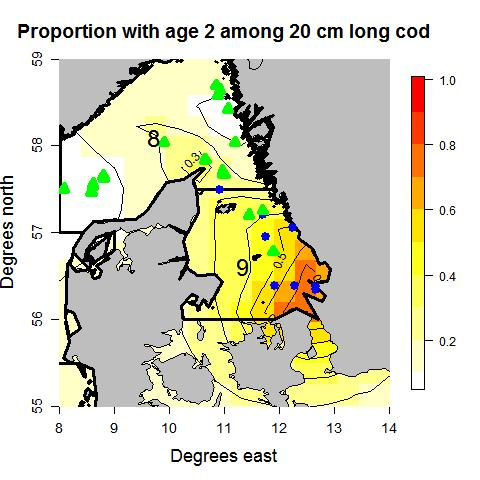
\includegraphics[scale=0.4]{figures/spatialALKQ1year2018RFA9Age2.jpeg}}
\captionsetup{font=small, width = 14.5cm}{
 \caption{Estimated proportion of age 1 and 2 year old cod of length 20 cm long in Skagerak. The green triangles and blue points are observations of one and two year old cod, respectively, which are in the length interval 19 cm to 21 cm. }\label{fig:proportionSkagerak}}
\end{figure}


Figures \ref{percentileBiascorrectedCIcod} gives estimates of indices of abundance for cod in years 2018 Q1 and for saithe in year 2017 Q3. Approximate 95\% confidence intervals from the bias-corrected bootstrap method for 200 bootstrap replication are estimated from the three ALK methods. The stratified procedure described in \ref{sec:datrasstratifiedbootstrap} is used in the sampling process to estimate bootstrap confidence intervals.   Figures \ref{percentileBiascorrectedCIcod}  shows that the resulting indices of abundance for cod and saithe turned out to be similar for all ALKs. IBTS is a complex multistage survey design, and since the ALKs are estimated from cluster-correlated data the resulting effective sample for estimating age-composition of fish would be lower than the number of fish measured \citep{ICES2013PICS3}. Hence, the ALKs are subject to large sampling errors. For example, the estimated percentage relative standard errors from the spatial ALKs for the plus group (6+) for cod are $>$ 25\%, suggesting high sampling error in the ALKs. Also, it should be remembered that DATRAS ALK is constant.   \citet{aanes2015efficient} showed that in such cases, and where only the variability of  length compositions are allowed for, the estimated age-distributions may appear to be more precise than they truly are since the ALK itself is subject to sampling errors, see for example the estimated relative standard standard errors for ages 2, and the older fish (4, 5 and 6+) for both species. 

As regards to which spatial ALK method to adopt, it is difficult to identify a method that gives the best performance over all age groups. While both methods seem to give reasonable estimates, the model based ALK generally gave shorter interval widths for both species. Uncertainty of relative abundance from the spatial ALK model is calculated using bootstrapping, as approximation of the joint distribution of the regression coefficient and spatial effect, in some cases, fails to account for the  negative correlations between ages. Also, estimating relative abundance at age and its precision from the spatial ALK model is computationally intensive. For these reasons we recommend the haul based ALK method for estimating age-distributions.

We also demonstrate the implications of using DATRAS bootstrap procedure for estimating the uncertainty around indices of abundance (see Figure \ref{DatrasStratified} in Supplementary Materials \ref{secAp:resultsdatrasALK}). Compared with the stratified bootstrap procedure, DATRAS bootstrap procedure gives an overestimation of the uncertainty for all age groups, suggesting that it is highly relevant to account for the variation in the data over large areas. 

\clearpage

\begin{figure*}[h!]
\centering
\begin{tabular}{@{}ccc@{}}
\subfloat[Cod in year 2018 Q1]{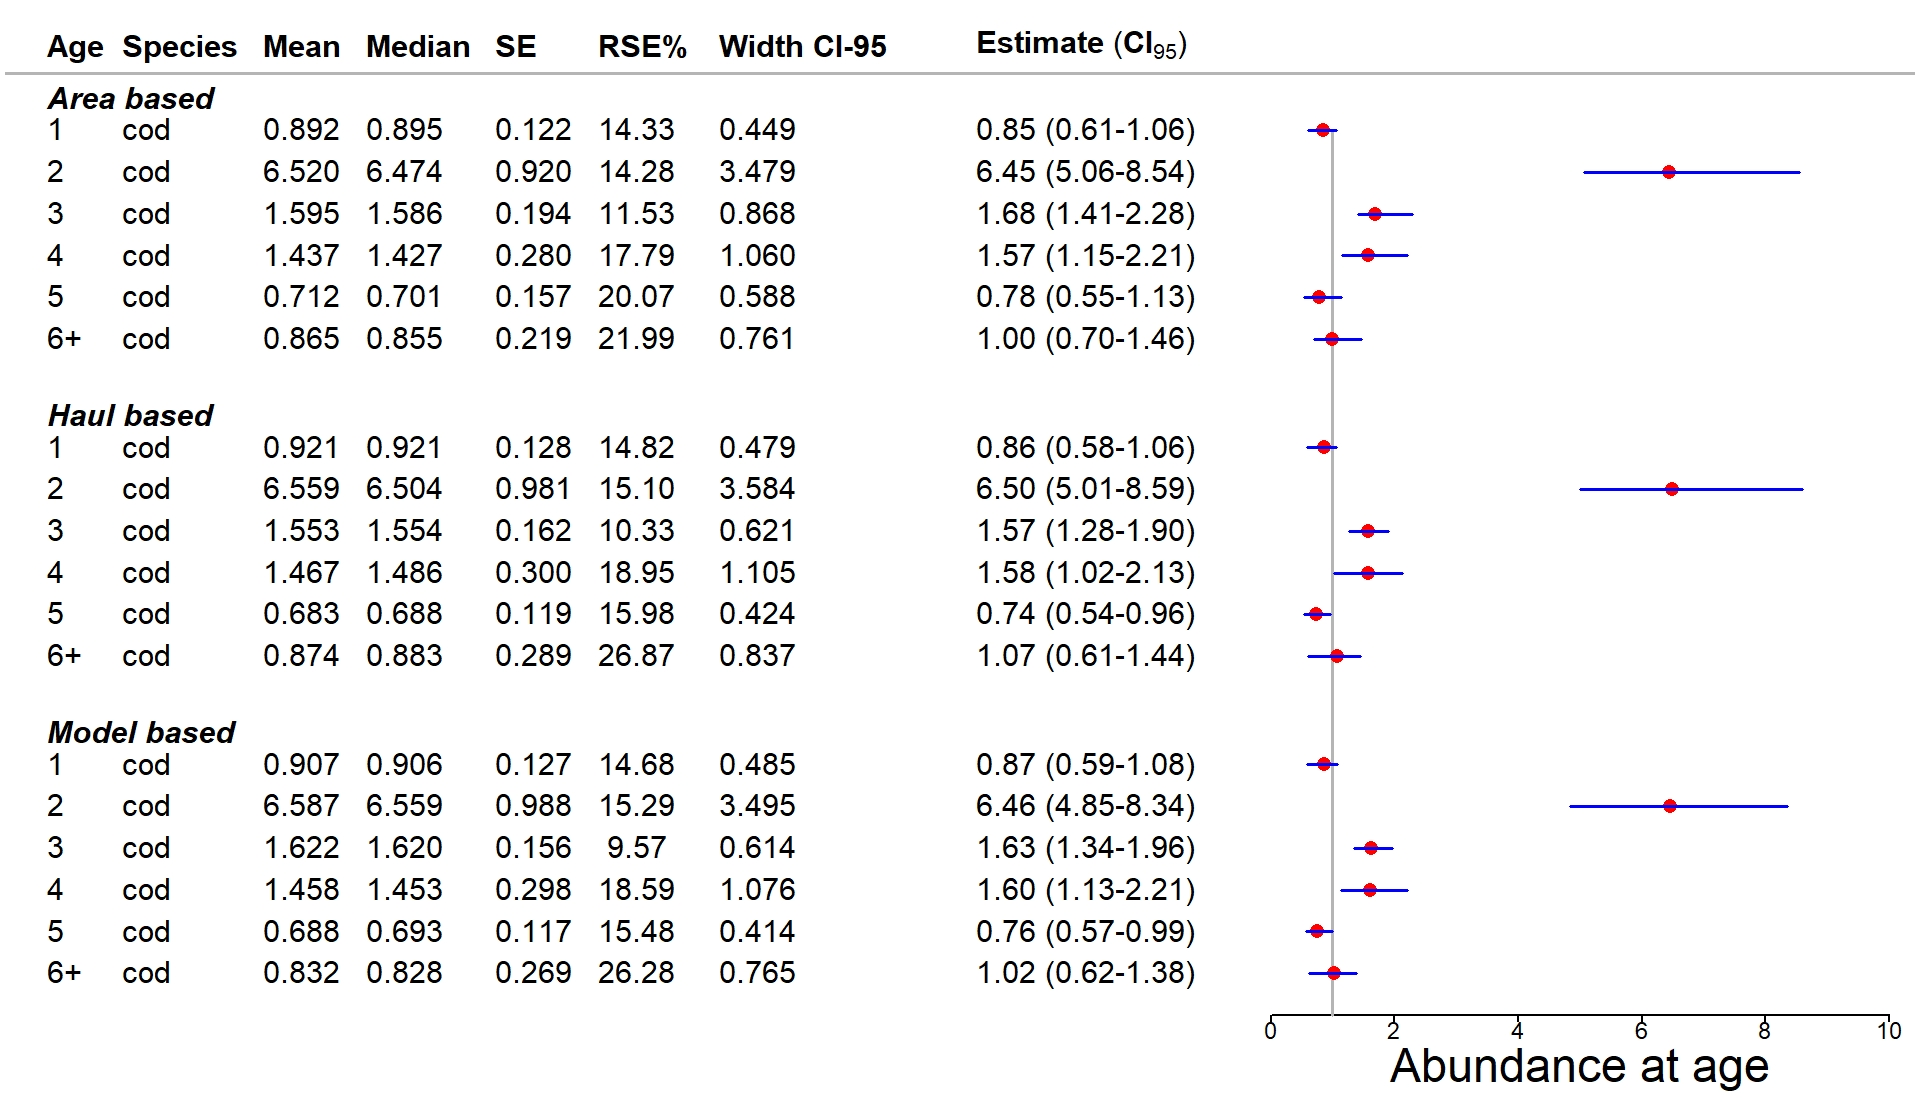
\includegraphics[width=0.95\textwidth]{figures/cod2018Q1BiasCorr.jpeg}} & \\
\subfloat[Saithe in year 2017 Q3]{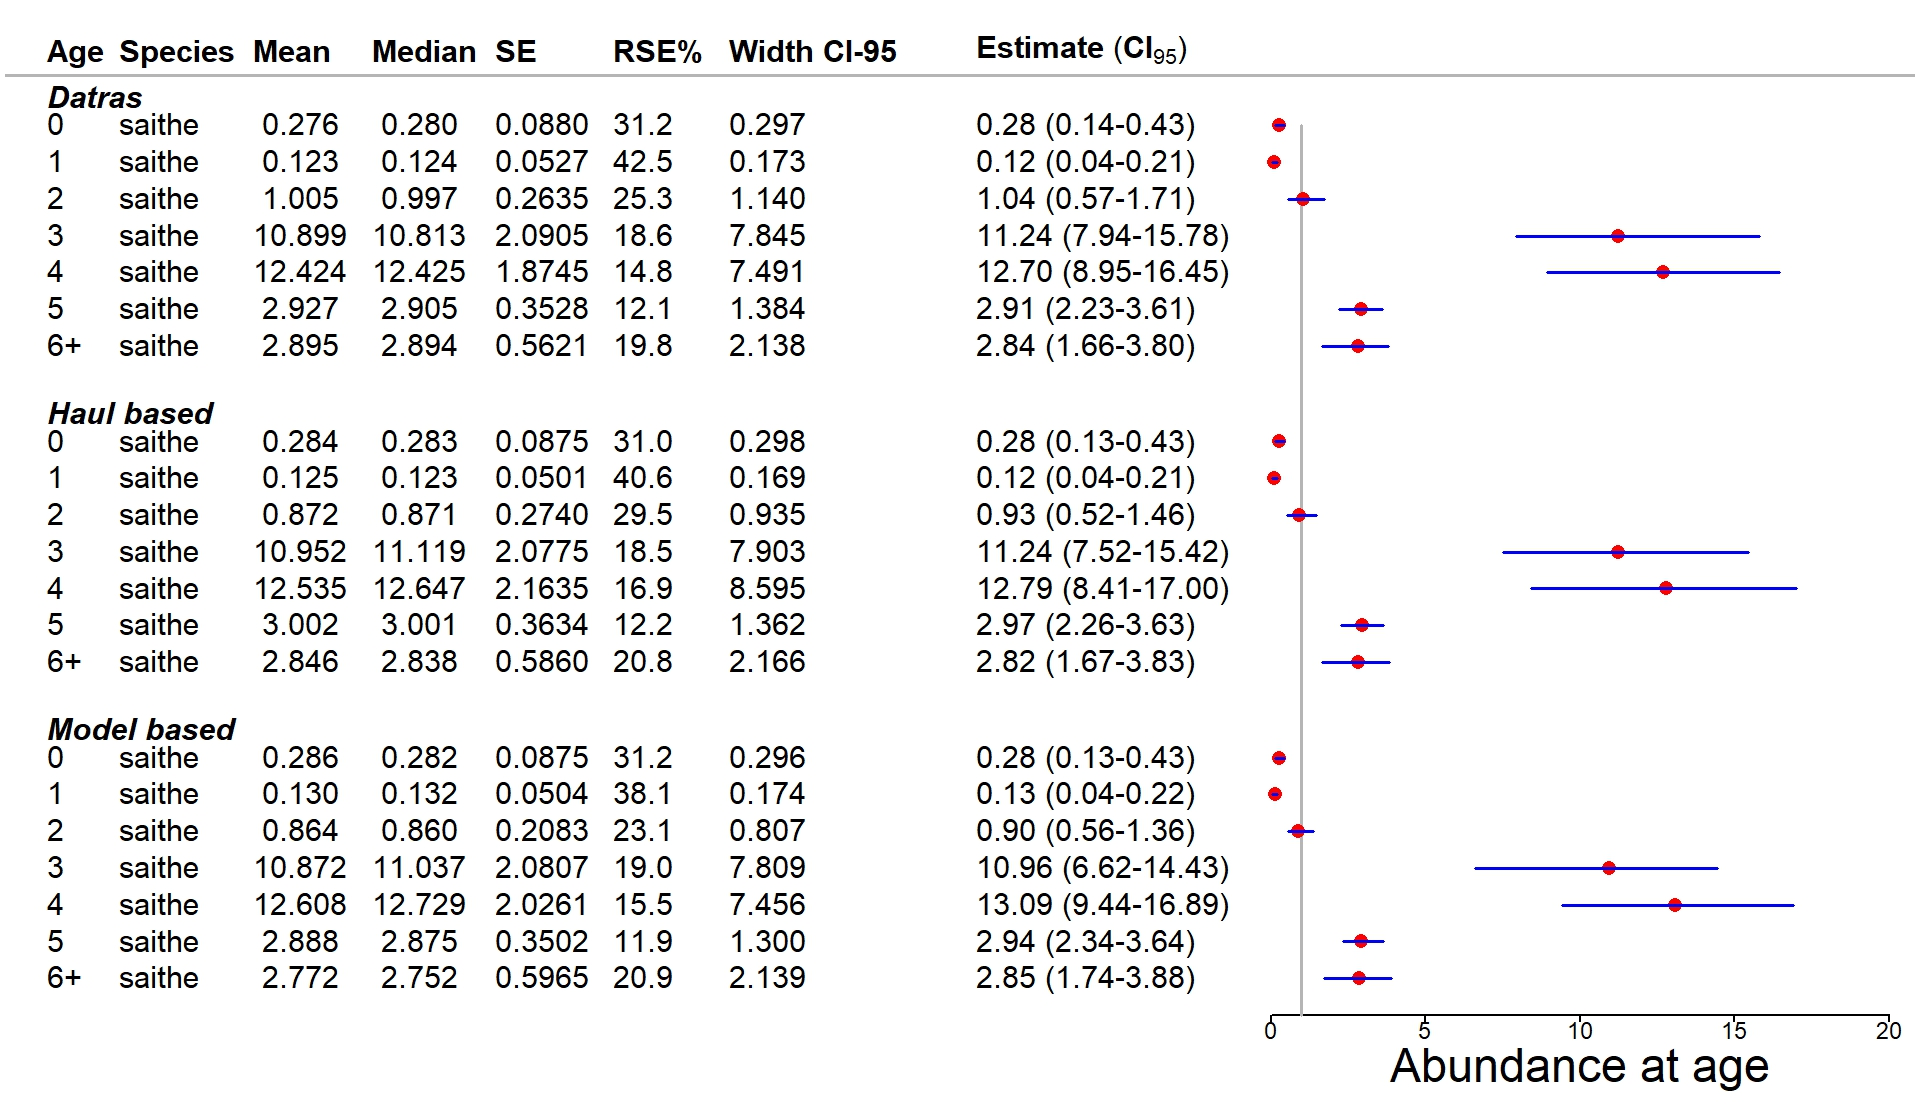
\includegraphics[width=0.95\textwidth]{figures/saithe2017Q3BiasCorr.jpeg}} &
\end{tabular}
\caption[]{Estimated confidence intervals ($\mathrm{CI}_{95}$) from bias-corrected  bootstrap method for cod in year 2018 Q1 and saithe in year 2017 Q3. Estimated indices of abundance (Estimate), and its standard error (SE), percentage relative standard error (RSE\%), bootstrap mean (Mean)  and Median estimates and the width of the confidence interval (Width CI-95) are also given.}
\label{percentileBiascorrectedCIcod}
\end{figure*} 

\clearpage
\subsection{Optimum sampling effort for North Sea Cod and Saithe}
\label{sec:optimumeffortresults}
To determine optimum sampling levels of otoliths for saithe and cod in the North Sea, ALKs are estimated using the haul based  method. As shown in Figure \ref{percentileBiascorrectedCIcod}  the haul based ALK and the model based ALK gave similar estimates of abundance indices and precision as both approaches are attempting to capture spatial variation in the data. But, the spatial model based ALK  is  quite complex, and model fitting would be computer-intensive since the model must be fitted for each bootstrap run and each simulated sampling procedure that mimics the real data collection procedure. For this reason, the model based ALK approach will not be used in this analysis. Also, the assumption of no difference in regional compositions of age-length structures is invalid,  as shown in Figure \ref{fig:proportionSkagerak},  so DATRAS ALK is not use for further analyses. The removal procedure for otolith sampling described in Section \ref{sec:optimizationsampling} is applied to data in year 2018 Q1 for cod and year 2017 Q3 for saithe. We sample one otolith per length group: 1 cm, 2 cm, 3 cm, 4 cm, 5 cm, 6 cm or 7 cm. Recall that the standardized IBTS sampling procedure is one otolith per length group for standard round fish as of year 2018 Q1, except for haddock and Norway Pout where 2 otoliths per cm is to be sampled (see Table \ref{tab:otolithsTable} in Supplementary Materials \ref{secAp:otolithappendix}). 

 Table \ref{codresults2018} compares estimates of relative  abundance ($\hat{\lambda}_{a}$) for the original sample of otolith data  with  bootstrap estimates of abundance indices  for the reduced sample of otolith data  ($\hat{\lambda}_{a}^{*}$) where a pair of otoliths are sampled from the following sampling procedures: 1 cm, 2 cm, 3 cm, 4 cm, 5 cm, 6 cm or 7 cm length group. The median estimated indices, estimated standard errors of the estimated indices of abundance from the reduced data, with  approximate bias-corrected bootstrap 95\% confidence intervals and percentage relative standard error are given for  $200$ simulations and $200$ bootstrap replication. Similar estimates are given for saithe in Table \ref{saitheresults2017}. A total of 1600 pairs of otoliths were sampled for cod in year 2018 Q1, while 2163 pairs of otoliths were sampled for saithe in year 2017 Q3 (see Table \ref{tab:data2018} in Supplementary Materials \ref{secAp:data}). The proportion of otoliths removed for cod from each of the sampling  procedures stated above is: 14.4\%, 28.6\%, 38.4\%, 44.5\%, 49.3\%, 52.6\% or 55.6\%, respectively, while for saithe the following proportions of otoliths are removed: 27.1\%, 48.9\%, 59.5\%, 65.6\%, 69.8\%, 73.1\% or 75.2\%, respectively.
  
 The results (Table \ref{codresults2018}) show that the difference between  ($\hat{\lambda}_{a}$) and ($\hat{\lambda}_{a}^{*}$) is marginal for all sampling procedures for ages 1-4. For the older fishes (ages 5 and 6+) this difference is clear, particularly for sampling procedures $\ge \ 5 \ \mathrm{cm}$. This is supported by the percentage relative standard error, but for all ages RSE\%$< 25\%$, suggesting that the variability in the estimates is low. A similar pattern emerges for satihe (Table \ref{saitheresults2017}), except for estimated relative abundance of age 2 saithe. It can be seen that the RSE\% is substantially larger than those of the neighbouring age groups, for example 1 or 3 year-olds. Almost all the RSE\% $>30\%$ for two-year olds, suggesting high variability in the parameter estimates (see $\hat{\lambda}_{a}$ and $\hat{\lambda}_{a}^{*}$ for age 2 saithe).  As shown in Figure \ref{fig:proportionSkagerak} the predicted probabilities of age-given-length of 2-year old saithe can overlap with younger fishes or older fishes, for example 3 or 4-year olds, and the proportion of otoliths of 2-year olds sampled during IBTS 2017 Q3 survey is a mere 3\% compared with 25\% and 35\% of 3-year and 4-year olds (see Table \ref{realdatacodandsaithe} in Supplementary Materials \ref{secAp:data}). And, given that a pair of otoliths (irrespective of age) is randomly selected from each of the following sampling procedures: 1 cm, 2 cm,...,7 cm, the older fishes (3 or 4-year olds) are more likely to be sampled, resulting in fewer samples utilised in the optimization procedure, and hence, higher variability in the estimates. Furthermore, the sampling variability in lengths of 2-year olds are high compared with 1-year olds and are comparable with 3-year and 4-year olds, so the standard error estimates of the estimated abundance indices may be dominated by this uncertainty. 

It can be seen also (Tables \ref{codresults2018} and \ref{saitheresults2017}) for the older fishes ($\geq 3-\mathrm{year \ olds}$) the confidence intervals are wider compared with the younger fishes. This could be for several reasons. The nonparametric bias-corrected bootstrap method is adopted for estimating confidence intervals of indices of abundance, and although this method has the advantage of correcting for the bias and skew of the sampling distribution of the data; accounting for some of the variability in the sampling distribution of the CPUE;  and does not assume any distribution for the data, there are some limitations of the bootstrap approach. The most important limitation is the assumption that the distribution of the data represented by the sample is a reasonable estimate of the population function from which the data are sampled. If this assumption is violated the random sampling  performed in the bootstrap procedure may add another level of sampling error, resulting in invalid statistical estimations \citep{haukoos2005advanced}. As discussed in Section \ref{overview} the selection of the trawling locations for IBTS surveys is semi-random where cruise leaders selects "clear" tow locations or "blind" tow locations if no clear tow exists by checking the proposed trawl track for hazardous seabed obstructions with acoustic methods. More recently, selection of tow locations is based on pre-proposed valid tow locations with start and end positions executed in the period 2000-2018. Hence, the lack of a fully randomized sampling process has the potential to result in biased estimates of parameters and their uncertainty. Additionally, prior to 2013, all nations were sampling 8 pairs of otoliths per 1 cm length group for our focal species (Table \ref{tab:otolithsTable} in Supplementary Materials \ref{secAp:otolithappendix}), and these samples could be acquired from, for example the first haul (or first few trawl hauls), resulting in an unrepresentative sample of the population. From 2013, some nations adopted the current sampling procedure outlined by ICES for IBTS 2018 surveys of 1 pair of otolith per 1 cm length group from each haul, while other nations continued with sampling 8 pairs of otoliths per 1 cm length group. So, bias was still introduced via the sampling  procedure. Another limitation of the bootstrap is the smaller the original sample the less likely it is to represent the entire population, thus the more difficult it becomes to compute valid confidence intervals. Note that the bootstrap relies heavily on the tails of the estimated sampling distribution when computing
confidence intervals, and using small samples may jeopardize the validity of this computation. As explained above, in 2017 Q3 data for 2-year old saithe, for example, 65 pairs of otoliths out of 2163 were sampled (a mere 3\%) and because of overlapping-age-length keys among neighbouring age groups, the probability of selecting 2-year olds is smaller, resulting in larger estimates of the variance, and hence wider confidence intervals. 

{\bf need to conclude on which sampling procedure is best based on estimated uncertainty (RSE\%), for example 5cm?}
 
%Furthermore, estimates of age 0 saithe lie on the boundary and estimated standard is 0. The sample size of 

%Aside from this, there is no evidence to suggest that the data represented by the sample is not a reasonable estimate of the population function.
%the probability of selecting a fish in a given length group is higher for the older age g
%  the number of otoliths sampled  Also    
%RSE\%$< 25\%$, suggesting that the variability in the estimates is low, the estimate of employed persons can be considered reliable enough for general use
%\clearpage
%Note that the nonparametric bootstrap method is advantageous  because it does not assume any distribution for the data, and it also accounts for some of the variability in the sampling distribution of the CPUE, however, there are some limitations of this method. The most important limitation is the assumption that the distribution of the data represented by the sample is a reasonable estimate of the population function from which the data are sampled. If this assumption is violated the random sampling  performed in the bootstrap procedure may add another level of sampling error, resulting in invalid statistical estimations \citep{haukoos2005advanced}. As discussed in Section \ref{overview} the selection of the trawling locations in IBTS is semi-random where cruise leaders selects "clear" tow locations or "blind" tow locations if no clear tow exists by checking the proposed trawl track for hazardous seabed obstructions with acoustic methods. More recently selection of tow locations is based on pre-proposed valid tow locations with start and end positions executed in the period 2000-2017. Hence, the lack of a fully randomized sampling process has the potential to result in biased estimates of parameters and their uncertainty. Random sampling performed in the bootstrap procedure also adds another level of potential sampling error, which is reflected in variation and biased estimates commonly performed in the bootstrap analysis. Note that the sampling distribution of the bootstrapped statistics is frequently not symmetric and computing point estimates from in this manner may reflect biased estimation from the samples. This can be seen in the estimated bootstrap mean values in Figure \ref{reduceresults}\\


\clearpage
 \begin{small}
\begin{table}[h!]
\centering
\setlength\tabcolsep{14.5pt} 
\captionsetup{font=small, width = 16.0cm}{
\caption{Estimated abundance ($\hat{\lambda}_{a}$) for cod from the original data in year 2018 Q1 compared with estimated abundance ($\hat{\lambda}_{a}^{*}$) from the reduced data for different sampling procedures of length groups ($l$). The estimated standard error of $\hat{\lambda}_{a}^{*}$ (SE($\hat{\lambda}_{a}^{*}$)) and the percentage relative standard error (RSE\%) are also given.}\label{codresults2018}}
\begin{footnotesize}
\begin{tabular}{clclclclclclcl}
  \hline \\ [0.3ex]
&  $l$ & $\hat{\lambda}_{a}$  & $\hat{\lambda}_{a}^{*}$ & (median) $\hat{\lambda}_{a}^{*}$ & SE($\hat{\lambda}_{a}^{*}$) & RSE\% &  CI-95 ($\hat{\lambda}_{a}^{*}$) \\ [1.0ex]
\hline \\
 \raisebox{1ex}{\bf age 1}  \\ [1.0ex]
&   1 cm & 0.863 &    0.866  & 0.867 &         0.00910& 1.051 & (0.84, 0.88)\\
&   2 cm & 0.863 &    0.866  & 0.866 &         0.00969& 1.119 & (0.84, 0.88)\\
&   3 cm & 0.863 &    0.858  & 0.862 &         0.02476& 2.886 & (0.81, 0.90) \\
&   4 cm & 0.863 &    0.854  & 0.855 &         0.02993& 3.507 & (0.81, 0.90) \\
&   5 cm & 0.863 &    0.848  & 0.850 &         0.03712& 4.379 & (0.81, 0.92)\\
&   6 cm & 0.863 &    0.858  & 0.858 &         0.03646& 4.249 & (0.80, 0.93)\\
&   7 cm & 0.863 &    0.856  & 0.857 &         0.03920& 4.582 & (0.80, 0.93)\\[1.5ex]

 \raisebox{1ex}{\bf age 2}  \\ [1.0ex]
&    1 cm & 6.496 &    6.485 & 6.483 &          0.02055& 0.317 & (6.47, 6.53)\\
&    2 cm & 6.496 &    6.485 & 6.486 &          0.01968& 0.303 & (6.46, 6.52)\\
&    3 cm & 6.496 &    6.503 & 6.506 &          0.05023& 0.772 & (6.38, 6.60)\\
&    4 cm & 6.496 &    6.498 & 6.498 &          0.05852& 0.901 & (6.39, 6.62)\\
&    5 cm & 6.496 &    6.507 & 6.505 &          0.07121& 1.094 & (6.36, 6.64)\\
&    6 cm & 6.496 &    6.510 & 6.512 &          0.07415& 1.139 & (6.34, 6.64)\\
&    7 cm & 6.496 &    6.491 & 6.496 &          0.08395& 1.293 & (6.33, 6.64)\\[1.5ex]

 \raisebox{1ex}{\bf age 3}  \\ [1.0ex]
&   1 cm & 1.571 &    1.574  & 1.567 &         0.06955& 4.418  & (1.46, 1.73)\\
&   2 cm & 1.571 &    1.579  & 1.575 &         0.06785& 4.429  & (1.45, 1.71)\\
&   3 cm & 1.571 &    1.559  & 1.556 &         0.09708& 6.228  & (1.41, 1.75)\\
&   4 cm & 1.571 &    1.641  & 1.640 &         0.10051& 6.124  & (1.41, 1.84)\\
&   5 cm & 1.571 &    1.627  & 1.622 &         0.12505& 7.686  & (1.31, 1.88)\\
&   6 cm & 1.571 &    1.643  & 1.640 &         0.12598& 7.670  & (1.31, 1.91)\\
&   7 cm & 1.571 &    1.753  & 1.763 &         0.13991& 7.979  & (1.44, 2.02) \\[1.5ex]

 \raisebox{1ex}{\bf age 4}  \\ [1.0ex]
&   1 cm & 1.584 &    1.603  & 1.597 &         0.12104& 7.550  & (1.37, 1.85)\\
&   2 cm & 1.584 &    1.592  & 1.593 &         0.11493& 7.218  & (1.37, 1.82)\\
&   3 cm & 1.584 &    1.610  & 1.603 &         0.14425& 8.960  & (1.31, 1.91)\\
&   4 cm & 1.584 &    1.571  & 1.570 &         0.15284& 9.729  & (1.31, 1.88)\\
&   5 cm & 1.584 &    1.585  & 1.583 &         0.15010& 9.468  & (1.32, 1.89)\\
&   6 cm & 1.584 &    1.588  & 1.600 &         0.15178& 9.560  & (1.26, 1.88)\\
&   7 cm & 1.584 &    1.503  & 1.518 &         0.16675& 11.094 & (1.38, 1.82) \\[1.5ex]

 \raisebox{1ex}{\bf age 5}  \\ [1.0ex]
&   1 cm & 0.742 &    0.740 & 0.738 &          0.10729& 14.504 & (0.56, 095)\\
&   2 cm & 0.742 &    0.744 & 0.724 &          0.11047& 14.848 & (0.57, 0.98)\\
&   3 cm & 0.742 &    0.764 & 0.760 &          0.11675& 15.287 & (0.55, 1.02)\\
&   4 cm & 0.742 &    0.752 & 0.735 &          0.11398& 15.158 & (0.58, 0.99)\\
&   5 cm & 0.742 &    0.814 & 0.805 &          0.12034& 14.789 & (0.53, 1.08)\\
&   6 cm & 0.742 &    0.782 & 0.766 &          0.10975& 14.043 & (0.57, 1.02)\\
&   7 cm & 0.742 &    0.813 & 0.790 &          0.12545& 15.425 & (0.59, 1.09) \\[1.5ex]

 \raisebox{1ex}{\bf age 6+}  \\ [1.0ex]
&   1 cm & 1.074 &    1.063 & 1.058 &          0.10489& 9.865  & (0.90, 1.28)\\
&   2 cm & 1.074 &    1.065 & 1.056 &          0.10657& 10.009 & (0.90, 1.29)\\
&   3 cm & 1.074 &    1.037 & 1.022 &          0.12215& 11.775 & (0.88, 1.25)\\
&   4 cm & 1.074 &    1.015 & 1.004 &          0.11855& 11.679 & (0.89, 1.24)\\
&   5 cm & 1.074 &    0.950 & 0.935 &          0.12210& 12.849 & (0.93, 1.21)\\
&   6 cm & 1.074 &    0.951 & 0.937 &          0.11562& 12.154 & (0.92, 1.19)\\
&   7 cm & 1.074 &    0.914 & 0.893 &          0.12577& 13.760 & (0.96, 1.18) \\[1.5ex]
  \hline \\
\end{tabular}
\end{footnotesize}
\end{table}
 \end{small}


\clearpage
 \begin{small}
\begin{table}[h!]
\centering
\setlength\tabcolsep{13.5pt} 
\captionsetup{font=small, width = 16cm}{
\caption{Estimated abundance ($\hat{\lambda}_{a}$) for saithe from the original data in year 2017 Q3 compared with estimated abundance ($\hat{\lambda}_{a}^{*}$) from the reduced data for different sampling procedures of length groups ($l$).}\label{saitheresults2017}}
\begin{footnotesize}
\begin{tabular}{clclclclclclcl}
  \hline \\ [0.3ex]
&  $l$ & $\hat{\lambda}_{a}$  & $\hat{\lambda}_{a}^{*}$ & (median) $\hat{\lambda}_{a}^{*}$  & SE($\hat{\lambda}_{a}^{*}$) & RSE\%&  CI-95 ($\hat{\lambda}_{a}^{*}$) \\ [1.0ex]
\hline \\
 \raisebox{1ex}{\bf age 0}  \\ [1.0ex]
&   1 cm & 0.282  &    0.282 &  0.282 &  0.00000 & 0.00 & (0.28, 0.28)\\
&   2 cm & 0.282  &    0.282 &  0.282 &  0.00000 & 0.00 & (0.28, 0.28)\\
&   3 cm & 0.282  &    0.288 &  0.295 &  0.00628 & 2.18 & (0.28, 0.29)\\
&   4 cm & 0.282  &    0.291 &  0.295 &  0.00578 & 1.99 & (0.28, 0.29)\\
&   5 cm & 0.282  &    0.282 &  0.282 &  0.00000 & 0.00 & (0.28, 0.28)\\
&   6 cm & 0.282  &    0.297 &  0.295 &  0.00949 & 3.19 & (0.28, 0.31)\\
&   7 cm & 0.282  &    0.290 &  0.295 &  0.00595 & 2.05 & (0.28, 0.29)\\[1.2ex]

 \raisebox{1ex}{\bf age 1}&  \\ [1.0ex]
&   1 cm & 0.123 &      0.123  & 0.123 & 0.00000  & 0.00 & (0.12, 0.12)\\
&   2 cm & 0.123 &      0.123  & 0.123 & 0.00000  & 0.00 & (0.12, 0.12)\\
&   3 cm & 0.123 &      0.117  & 0.111 & 0.00628  & 5.36 & (0.11, 0.12)\\
&   4 cm & 0.123 &      0.117  & 0.115 & 0.00641  & 5.47 & (0.11, 0.13) \\
&   5 cm & 0.123 &      0.125  & 0.126 & 0.00139  & 1.11 & (0.12, 0.13) \\
&   6 cm & 0.123 &      0.112  & 0.114 & 0.00942  & 8.43 & (0.11, 0.13)\\
&   7 cm & 0.123 &      0.115  & 0.114 & 0.00630  & 5.46 & (0.11, 0.13)\\[1.2ex]

\raisebox{1ex}{\bf age 2} &  \\ [1.0ex]
&   1 cm & 0.929 &    0.917  & 0.913 &         0.17774& 19.39 & (0.58, 1.25)\\
&   2 cm & 0.929 &    0.892  & 0.856 &         0.28437& 31.89 & (0.47, 1.50) \\
&   3 cm & 0.929 &    0.985  & 0.918 &         0.33392& 33.90 & (0.51, 1.65)\\
&   4 cm & 0.929 &    0.982  & 0.922 &         0.33738& 34.36 & (0.48, 1.55)\\
&   5 cm & 0.929 &    1.003  & 0.948 &         0.34661& 34.56 & (0.50, 1.61)\\
&   6 cm & 0.929 &    0.945  & 0.892 &         0.33643& 35.60 & (0.49, 1.77)\\
&   7 cm & 0.929 &    0.982  & 0.929 &         0.33668& 34.28 & (0.42, 1.62)\\[1.2ex]

 \raisebox{1ex}{\bf age 3} \\ [1.0ex]
&   1 cm & 11.238  &  11.272 & 11.300 &          0.53160& 4.72  & (10.30, 12.15)\\
&   2 cm & 11.238  &  11.161 & 11.163 &          0.93489& 8.38  & (9.56, 13.11)\\
&   3 cm & 11.238  &  11.091 & 11.173 &          1.17954& 10.64 & (9.15, 13.39)\\
&   4 cm & 11.238  &  10.903 & 11.022 &          1.05854& 9.71  & (9.45, 13.27)\\
&   5 cm & 11.238  &  10.857 & 10.718 &          1.12152& 10.33 & (9.16, 12.95)\\
&   6 cm & 11.238  &  10.937 & 10.914 &          1.10301& 10.09 & (9.77, 12.88)\\
&   7 cm & 11.238  &  10.724 & 10.658 &          1.04157& 9.71  & (8.80, 13.07)\\[1.5ex]

 \raisebox{1ex}{\bf age 4} &  \\ [1.0ex]
 &  1 cm & 12.789 &   12.773 & 12.793 &          0.52290& 4.09 & (11.89, 13.74) \\
 &  2 cm & 12.789 &   12.874 & 12.903 &          0.91838& 7.13 & (10.80, 14.54) \\
 &  3 cm & 12.789 &   12.877 & 12.771 &          1.14444& 8.89 & (10.76, 14.84) \\
 &  4 cm & 12.789 &   13.019 & 13.033 &          1.09987& 8.45 & (10.69, 15.09) \\
 &  5 cm & 12.789 &   13.033 & 13.114 &          1.15195& 8.84 & (10.51, 15.25) \\
 &  6 cm & 12.789 &   13.111 & 13.056 &          1.09241& 8.33 & (10.57, 15.13) \\
 &  7 cm & 12.789 &   13.278 & 13.267 &          1.07854& 8.12 & (10.23, 15.64) \\[1.2ex]

 \raisebox{1ex}{age 5}  \\ [1.0ex]
&  1 cm  & 2.971 &     2.967   & 2.962 &        0.12220& 4.12  & (2.76, 3.24) \\
&   2 cm & 2.971 &     3.036   & 3.006 &        0.29591& 9.75  & (2.48, 3.58) \\
&   3 cm & 2.971 &     2.970   & 2.945 &        0.29382& 9.89  & (2.47, 3.61) \\
&   4 cm & 2.971 &     3.045   & 3.040 &        0.38412& 12.61 & (2.31, 3.99) \\
&   5 cm & 2.971 &     3.077   & 2.996 &        0.43326& 14.08 & (2.31, 3.87)\\
&   6 cm & 2.971 &     2.936   & 2.898 &        0.38625& 13.16 & (2.23, 3.77)\\
&   7 cm & 2.971 &     2.971   & 2.938 &        0.42992& 14.14 & (2.12, 3.81)\\[1.2ex]

 \raisebox{1ex}{\bf age 6+} &   \\ [1.0ex]
&   1 cm & 2.819  &   2.817 & 2.820 &          0.05126& 1.82 & (2.73, 2.90) \\
&   2 cm & 2.819  &   2.783 & 2.782 &          0.08525& 3.06 & (2.70, 2.94) \\
&   3 cm & 2.819  &   2.823 & 2.821 &          0.11729& 4.15 & (2.64, 3.04) \\
&   4 cm & 2.819  &   2.794 & 2.796 &          0.12590& 4.15 & (2.61, 3.05) \\
&   5 cm & 2.819  &   2.775 & 2.782 &          0.13938& 5.02 & (2.54, 3.02) \\
&   6 cm & 2.819  &   2.813 & 2.803 &          0.14435& 5.13 & (2.53, 3.12)  \\
&   7 cm & 2.819  &   2.790 & 2.794 &          0.15922& 5.71 & (2.54, 3.06)  \\[0.1ex]
   \hline \\
\end{tabular}
\end{footnotesize}
\end{table}
 \end{small}
 
%
%\clearpage
% \begin{small}
%\begin{table}[h!]
%\centering
%\setlength\tabcolsep{18.5pt} 
%\captionsetup{font=small, width = 15.5cm}{
%\caption{Estimated abundance ($\hat{\lambda}_{a}$) for cod from the original data in year 2018 Q1 compared with estimated abundance ($\hat{\lambda}_{a}^{*}$) from the reduced data for different sampling procedures of length groups ($l$). The estimated standard error of $\hat{\lambda}_{a}^{*}$ (SE($\hat{\lambda}_{a}^{*}$)) and the percentage relative standard error (RSE\%) are also given.}\label{codresults2018}}
%\begin{footnotesize}
%\begin{tabular}{clclclclcl}
%  \hline \\ [0.3ex]
%&  $l$ & $\hat{\lambda}_{a}$  & $\hat{\lambda}_{a}^{*}$ & SE($\hat{\lambda}_{a}^{*}$) & RSE\% &  CI-95 ($\hat{\lambda}_{a}^{*}$) \\ [1.0ex]
%\hline \\
% \raisebox{1ex}{\bf age 1}  \\ [1.0ex]
%&   1 cm & 0.863 &    0.866  &          0.00910& 1.051 & (0.84, 0.88)\\
%&   2 cm & 0.863 &    0.866  &          0.00969& 1.119 & (0.84, 0.88)\\
%&   3 cm & 0.863 &    0.858  &          0.02476& 2.886 & (0.81, 0.90) \\
%&   4 cm & 0.863 &    0.854  &          0.02993& 3.507 & (0.81, 0.90) \\
%&   5 cm & 0.863 &    0.848  &          0.03712& 4.379 & (0.81, 0.92)\\
%&   6 cm & 0.863 &    0.858  &          0.03646& 4.249 & (0.80, 0.93)\\
%&   7 cm & 0.863 &    0.856  &          0.03920& 4.582 & (0.80, 0.93)\\[1.5ex]
%
% \raisebox{1ex}{\bf age 2}  \\ [1.0ex]
%&    1 cm & 6.496 &    6.485 &           0.02055& 0.317 & (6.47, 6.53)\\
%&    2 cm & 6.496 &    6.485 &           0.01968& 0.303 & (6.46, 6.52)\\
%&    3 cm & 6.496 &    6.503 &           0.05023& 0.772 & (6.38, 6.60)\\
%&    4 cm & 6.496 &    6.498 &           0.05852& 0.901 & (6.39, 6.62)\\
%&    5 cm & 6.496 &    6.507 &           0.07121& 1.094 & (6.36, 6.64)\\
%&    6 cm & 6.496 &    6.510 &           0.07415& 1.139 & (6.34, 6.64)\\
%&    7 cm & 6.496 &    6.491 &           0.08395& 1.293 & (6.33, 6.64)\\[1.5ex]
%
% \raisebox{1ex}{\bf age 3}  \\ [1.0ex]
%&   1 cm & 1.571 &    1.574  &          0.06955& 4.418  & (1.46, 1.73)\\
%&   2 cm & 1.571 &    1.579  &          0.06785& 4.429  & (1.45, 1.71)\\
%&   3 cm & 1.571 &    1.559  &          0.09708& 6.228  & (1.41, 1.75)\\
%&   4 cm & 1.571 &    1.641  &          0.10051& 6.124  & (1.41, 1.84)\\
%&   5 cm & 1.571 &    1.627  &          0.12505& 7.686  & (1.31, 1.88)\\
%&   6 cm & 1.571 &    1.643  &          0.12598& 7.670  & (1.31, 1.91)\\
%&   7 cm & 1.571 &    1.753  &          0.13991& 7.979  & (1.44, 2.02) \\[1.5ex]
%
% \raisebox{1ex}{\bf age 4}  \\ [1.0ex]
%&   1 cm & 1.584 &    1.603  &          0.12104& 7.550  & (1.37, 1.85)\\
%&   2 cm & 1.584 &    1.592  &          0.11493& 7.218  & (1.37, 1.82)\\
%&   3 cm & 1.584 &    1.610  &          0.14425& 8.960  & (1.31, 1.91)\\
%&   4 cm & 1.584 &    1.571  &          0.15284& 9.729  & (1.31, 1.88)\\
%&   5 cm & 1.584 &    1.585  &          0.15010& 9.468  & (1.32, 1.89)\\
%&   6 cm & 1.584 &    1.588  &          0.15178& 9.560  & (1.26, 1.88)\\
%&   7 cm & 1.584 &    1.503  &          0.16675& 11.094 & (1.38, 1.82) \\[1.5ex]
%
% \raisebox{1ex}{\bf age 5}  \\ [1.0ex]
%&   1 cm & 0.742 &    0.740 &           0.10729& 14.504 & (0.56, 095)\\
%&   2 cm & 0.742 &    0.744 &           0.11047& 14.848 & (0.57, 0.98)\\
%&   3 cm & 0.742 &    0.764 &           0.11675& 15.287 & (0.55, 1.02)\\
%&   4 cm & 0.742 &    0.752 &           0.11398& 15.158 & (0.58, 0.99)\\
%&   5 cm & 0.742 &    0.814 &           0.12034& 14.789 & (0.53, 1.08)\\
%&   6 cm & 0.742 &    0.782 &           0.10975& 14.043 & (0.57, 1.02)\\
%&   7 cm & 0.742 &    0.813 &           0.12545& 15.425 & (0.59, 1.09) \\[1.5ex]
%
% \raisebox{1ex}{\bf age 6+}  \\ [1.0ex]
%&   1 cm & 1.074 &    1.063 &           0.10489& 9.865  & (0.90, 1.28)\\
%&   2 cm & 1.074 &    1.065 &           0.10657& 10.009 & (0.90, 1.29)\\
%&   3 cm & 1.074 &    1.037 &           0.12215& 11.775 & (0.88, 1.25)\\
%&   4 cm & 1.074 &    1.015 &           0.11855& 11.679 & (0.89, 1.24)\\
%&   5 cm & 1.074 &    0.950 &           0.12210& 12.849 & (0.93, 1.21)\\
%&   6 cm & 1.074 &    0.951 &           0.11562& 12.154 & (0.92, 1.19)\\
%&   7 cm & 1.074 &    0.914 &           0.12577& 13.760 & (0.96, 1.18) \\[1.5ex]
%  \hline \\
%\end{tabular}
%\end{footnotesize}
%\end{table}
% \end{small}
%

% \begin{small}
%\begin{table}[h!]
%\centering
%\setlength\tabcolsep{15.5pt} 
%\captionsetup{font=small, width = 15cm}{
%\caption{Estimated abundance ($\hat{\lambda}_{a}$) for saithe from the original data in year 2017 Q3 compared with estimated abundance ($\hat{\lambda}_{a}^{*}$) from the reduced data for different sampling procedures of length groups ($l$).}\label{saitheresults2017}}
%\begin{footnotesize}
%\begin{tabular}{clclclclclclcl}
%  \hline \\ [0.3ex]
%&  $l$ & $\hat{\lambda}_{a}$  & $\hat{\lambda}_{a}^{*}$  & SE($\hat{\lambda}_{a}^{*}$) & RSE\%&  CI-95 ($\hat{\lambda}_{a}^{*}$) \\ [1.0ex]
%\hline \\
% \raisebox{1ex}{\bf age 0}  \\ [1.0ex]
%&   1 cm & 0.282  &    0.282 &           0.00000& 0.00 & (0.28, 0.28)\\
%&   2 cm & 0.282  &    0.282 &           0.00000& 0.00 & (0.28, 0.28)\\
%&   3 cm & 0.282  &    0.288 &           0.00628& 2.18 & (0.28, 0.29)\\
%&   4 cm & 0.282  &    0.291 &           0.00578& 1.99 & (0.28, 0.29)\\
%&   5 cm & 0.282  &    0.282 &           0.00000& 0.00 & (0.28, 0.28)\\
%&   6 cm & 0.282  &    0.297 &           0.00949& 3.19 & (0.28, 0.31)\\
%&   7 cm & 0.282  &    0.290 &           0.00595& 2.05 & (0.28, 0.29)\\[1.2ex]
%
% \raisebox{1ex}{\bf age 1}&  \\ [1.0ex]
%&   1 cm & 0.123 &      0.123  &          0.00000& 0.00 & (0.12, 0.12)\\
%&   2 cm & 0.123 &      0.123  &          0.00000& 0.00 & (0.12, 0.12)\\
%&   3 cm & 0.123 &      0.117  &          0.00628& 5.36 & (0.11, 0.12)\\
%&   4 cm & 0.123 &      0.117  &          0.00641& 5.47 & (0.11, 0.13) \\
%&   5 cm & 0.123 &      0.125  &          0.00139& 1.11 & (0.12, 0.13) \\
%&   6 cm & 0.123 &      0.112  &          0.00942& 8.43 & (0.11, 0.13)\\
%&   7 cm & 0.123 &      0.115  &          0.00630& 5.46 & (0.11, 0.13)\\[1.2ex]
%
%\raisebox{1ex}{\bf age 2} &  \\ [1.0ex]
%&   1 cm & 0.929 &    0.917  &          0.17774& 19.39 & (0.58, 1.25)\\
%&   2 cm & 0.929 &    0.892  &          0.28437& 31.89 & (0.47, 1.50) \\
%&   3 cm & 0.929 &    0.985  &          0.33392& 33.90 & (0.51, 1.65)\\
%&   4 cm & 0.929 &    0.982  &          0.33738& 34.36 & (0.48, 1.55)\\
%&   5 cm & 0.929 &    1.003  &          0.34661& 34.56 & (0.50, 1.61)\\
%&   6 cm & 0.929 &    0.945  &          0.33643& 35.60 & (0.49, 1.77)\\
%&   7 cm & 0.929 &    0.982  &          0.33668& 34.28 & (0.42, 1.62)\\[1.2ex]
%
% \raisebox{1ex}{\bf age 3} \\ [1.0ex]
%&   1 cm & 11.238  &  11.272 &           0.53160& 4.72  & (10.30, 12.15)\\
%&   2 cm & 11.238  &  11.161 &           0.93489& 8.38  & (9.56, 13.11)\\
%&   3 cm & 11.238  &  11.091 &           1.17954& 10.64 & (9.15, 13.39)\\
%&   4 cm & 11.238  &  10.903 &           1.05854& 9.71  & (9.45, 13.27)\\
%&   5 cm & 11.238  &  10.857 &           1.12152& 10.33 & (9.16, 12.95)\\
%&   6 cm & 11.238  &  10.937 &           1.10301& 10.09 & (9.77, 12.88)\\
%&   7 cm & 11.238  &  10.724 &           1.04157& 9.71  & (8.80, 13.07)\\[1.5ex]
%
% \raisebox{1ex}{\bf age 4} &  \\ [1.0ex]
% &  1 cm & 12.789 &   12.773 &           0.52290& 4.09 & (11.89, 13.74) \\
% &  2 cm & 12.789 &   12.874 &           0.91838& 7.13 & (10.80, 14.54) \\
% &  3 cm & 12.789 &   12.877 &           1.14444& 8.89 & (10.76, 14.84) \\
% &  4 cm & 12.789 &   13.019 &           1.09987& 8.45 & (10.69, 15.09) \\
% &  5 cm & 12.789 &   13.033 &           1.15195& 8.84 & (10.51, 15.25) \\
% &  6 cm & 12.789 &   13.111 &           1.09241& 8.33 & (10.57, 15.13) \\
% &  7 cm & 12.789 &   13.278 &           1.07854& 8.12 & (10.23, 15.64) \\[1.2ex]
%
% \raisebox{1ex}{age 5}  \\ [1.0ex]
%&  1 cm  & 2.971 &     2.967   &         0.12220& 4.12  & (2.76, 3.24) \\
%&   2 cm & 2.971 &     3.036   &         0.29591& 9.75  & (2.48, 3.58) \\
%&   3 cm & 2.971 &     2.970   &         0.29382& 9.89  & (2.47, 3.61) \\
%&   4 cm & 2.971 &     3.045   &         0.38412& 12.61 & (2.31, 3.99) \\
%&   5 cm & 2.971 &     3.077   &         0.43326& 14.08 & (2.31, 3.87)\\
%&   6 cm & 2.971 &     2.936   &         0.38625& 13.16 & (2.23, 3.77)\\
%&   7 cm & 2.971 &     2.971   &         0.42992& 14.14 & (2.12, 3.81)\\[1.2ex]
%
% \raisebox{1ex}{\bf age 6+} &   \\ [1.0ex]
%&   1 cm & 2.819  &   2.817 &           0.05126& 1.82 & (2.73, 2.90) \\
%&   2 cm & 2.819  &   2.783 &           0.08525& 3.06 & (2.70, 2.94) \\
%&   3 cm & 2.819  &   2.823 &           0.11729& 4.15 & (2.64, 3.04) \\
%&   4 cm & 2.819  &   2.794 &           0.12590& 4.15 & (2.61, 3.05) \\
%&   5 cm & 2.819  &   2.775 &           0.13938& 5.02 & (2.54, 3.02) \\
%&   6 cm & 2.819  &   2.813 &           0.14435& 5.13 & (2.53, 3.12)  \\
%&   7 cm & 2.819  &   2.790 &           0.15922& 5.71 & (2.54, 3.06)  \\[0.1ex]
%   \hline \\
%\end{tabular}
%\end{footnotesize}
%\end{table}
% \end{small}
% 


%
%
%\clearpage
% \begin{small}
%\begin{table}[h!]
%\centering
%\setlength\tabcolsep{15.5pt} 
%\captionsetup{font=small, width = 16cm}{
%\caption{Estimated abundance ($\lambda_{a}$) for cod from the original data in year 2018 Q1 compared with estimated abundance ($\lambda_{a}^{*}$) from the reduced data for different sampling procedures of length groups ($l$). The estimated standard error of $\hat{\lambda}_{a}^{*}$ (SE($\hat{\lambda}_{a}^{*}$)) and the percentage relative standard error (RSE\%) are also given.}\label{codresults2018}}
%\begin{footnotesize}
%\begin{tabular}{clclclclcl}
%  \hline \\ [0.3ex]
%&  $l$ & $\hat{\lambda}_{a}$ & \thead{Otoliths\\ removed} & $\hat{\lambda}_{a}^{*}$ & SE($\hat{\lambda}_{a}^{*}$) & RSE\% &  CI-95 ($\hat{\lambda}_{a}^{*}$) \\ [1.0ex]
%\hline \\
% \raisebox{1ex}{\bf age 1}  \\ [1.0ex]
%&   1 cm & 0.863 &   231 & 0.866  &          0.00910& 1.051 & (0.84, 0.88)\\
%&   2 cm & 0.863 &   457 & 0.866  &          0.00969& 1.119 & (0.84, 0.88)\\
%&   3 cm & 0.863 &   615 & 0.858  &          0.02476& 2.886 & (0.81, 0.90) \\
%&   4 cm & 0.863 &   712 & 0.854  &          0.02993& 3.507 & (0.81, 0.90) \\
%&   5 cm & 0.863 &   788 & 0.848  &          0.03712& 4.379 & (0.81, 0.92)\\
%&   6 cm & 0.863 &   841 & 0.858  &          0.03646& 4.249 & (0.80, 0.93)\\
%&   7 cm & 0.863 &   889 & 0.856  &          0.03920& 4.582 & (0.80, 0.93)\\[1.5ex]
%
% \raisebox{1ex}{\bf age 2}  \\ [1.0ex]
%&    1 cm & 6.496 &  231 &  6.485 &           0.02055& 0.317 & (6.47, 6.53)\\
%&    2 cm & 6.496 &  457 &  6.485 &           0.01968& 0.303 & (6.46, 6.52)\\
%&    3 cm & 6.496 &  615 &  6.503 &           0.05023& 0.772 & (6.38, 6.60)\\
%&    4 cm & 6.496 &  712 &  6.498 &           0.05852& 0.901 & (6.39, 6.62)\\
%&    5 cm & 6.496 &  788 &  6.507 &           0.07121& 1.094 & (6.36, 6.64)\\
%&    6 cm & 6.496 &  841 &  6.510 &           0.07415& 1.139 & (6.34, 6.64)\\
%&    7 cm & 6.496 &  889 &  6.491 &           0.08395& 1.293 & (6.33, 6.64)\\[1.5ex]
%
% \raisebox{1ex}{\bf age 3}  \\ [1.0ex]
%&   1 cm & 1.571 &  213 &  1.574  &          0.06955& 4.418  & (1.46, 1.73)\\
%&   2 cm & 1.571 &  457 &  1.579  &          0.06785& 4.429  & (1.45, 1.71)\\
%&   3 cm & 1.571 &  615 &  1.559  &          0.09708& 6.228  & (1.41, 1.75)\\
%&   4 cm & 1.571 &  712 &  1.641  &          0.10051& 6.124  & (1.41, 1.84)\\
%&   5 cm & 1.571 &  788 &  1.627  &          0.12505& 7.686  & (1.31, 1.88)\\
%&   6 cm & 1.571 &  841 &  1.643  &          0.12598& 7.670  & (1.31, 1.91)\\
%&   7 cm & 1.571 &  889 &  1.753  &          0.13991& 7.979  & (1.44, 2.02) \\[1.5ex]
%
% \raisebox{1ex}{\bf age 4}  \\ [1.0ex]
%&   1 cm & 1.584 &  213 &  1.603  &          0.12104& 7.550  & (1.37, 1.85)\\
%&   2 cm & 1.584 &  457 &  1.592  &          0.11493& 7.218  & (1.37, 1.82)\\
%&   3 cm & 1.584 &  615 &  1.610  &          0.14425& 8.960  & (1.31, 1.91)\\
%&   4 cm & 1.584 &  712 &  1.571  &          0.15284& 9.729  & (1.31, 1.88)\\
%&   5 cm & 1.584 &  788 &  1.585  &          0.15010& 9.468  & (1.32, 1.89)\\
%&   6 cm & 1.584 &  841 &  1.588  &          0.15178& 9.560  & (1.26, 1.88)\\
%&   7 cm & 1.584 &  889 &  1.503  &          0.16675& 11.094 & (1.38, 1.82) \\[1.5ex]
%
% \raisebox{1ex}{\bf age 5}  \\ [1.0ex]
%&   1 cm & 0.742 &  213 &  0.740 &           0.10729& 14.504 & (0.56, 095)\\
%&   2 cm & 0.742 &  457 &  0.744 &           0.11047& 14.848 & (0.57, 0.98)\\
%&   3 cm & 0.742 &  615 &  0.764 &           0.11675& 15.287 & (0.55, 1.02)\\
%&   4 cm & 0.742 &  712 &  0.752 &           0.11398& 15.158 & (0.58, 0.99)\\
%&   5 cm & 0.742 &  788 &  0.814 &           0.12034& 14.789 & (0.53, 1.08)\\
%&   6 cm & 0.742 &  841 &  0.782 &           0.10975& 14.043 & (0.57, 1.02)\\
%&   7 cm & 0.742 &  889 &  0.813 &           0.12545& 15.425 & (0.59, 1.09) \\[1.5ex]
%
% \raisebox{1ex}{\bf age 6+}  \\ [1.0ex]
%&   1 cm & 1.074 &  231 &  1.063 &           0.10489& 9.865  & (0.90, 1.28)\\
%&   2 cm & 1.074 &  457 &  1.065 &           0.10657& 10.009 & (0.90, 1.29)\\
%&   3 cm & 1.074 &  615 &  1.037 &           0.12215& 11.775 & (0.88, 1.25)\\
%&   4 cm & 1.074 &  712 &  1.015 &           0.11855& 11.679 & (0.89, 1.24)\\
%&   5 cm & 1.074 &  788 &  0.950 &           0.12210& 12.849 & (0.93, 1.21)\\
%&   6 cm & 1.074 &  841 &  0.951 &           0.11562& 12.154 & (0.92, 1.19)\\
%&   7 cm & 1.074 &  889 &  0.914 &           0.12577& 13.760 & (0.96, 1.18) \\[1.5ex]
%  \hline \\
%\end{tabular}
%\end{footnotesize}
%\end{table}
% \end{small}
%
%
%\clearpage
% \begin{small}
%\begin{table}[h!]
%\centering
%\setlength\tabcolsep{13.5pt} 
%\captionsetup{font=small, width = 16.5cm}{
%\caption{Estimated abundance ($\lambda_{a}$) for saithe from the original data in year 2017 Q3 compared with estimated abundance ($\lambda_{a}^{*}$) from the reduced data for different sampling procedures of length groups ($l$).}\label{saitheresults2017}}
%\begin{footnotesize}
%\begin{tabular}{clclclclcl}
%  \hline \\ [0.3ex]
%&  $l$ & $\hat{\lambda}_{a}$ & \thead{Otoliths  removed} & $\hat{\lambda}_{a}^{*}$ & SE($\hat{\lambda}_{a}^{*}$) & RSE\%&  CI-95 ($\hat{\lambda}_{a}^{*}$) \\ [1.0ex]
%\hline \\
% \raisebox{1ex}{\bf age 0}  \\ [1.0ex]
%&   1 cm & 0.282  &  586  &  0.282 &           0.00000& 0.00 & (0.28, 0.28)\\
%&   2 cm & 0.282  &  1057 &  0.282 &           0.00000& 0.00 & (0.28, 0.28)\\
%&   3 cm & 0.282  &  1287 &  0.288 &           0.00628& 2.18 & (0.28, 0.29)\\
%&   4 cm & 0.282  &  1420 &  0.291 &           0.00578& 1.99 & (0.28, 0.29)\\
%&   5 cm & 0.282  &  1509 &  0.282 &           0.00000& 0.00 & (0.28, 0.28)\\
%&   6 cm & 0.282  &  1581 &  0.297 &           0.00949& 3.19 & (0.28, 0.31)\\
%&   7 cm & 0.282  &  1626 &  0.290 &           0.00595& 2.05 & (0.28, 0.29)\\[1.2ex]
%
% \raisebox{1ex}{\bf age 1}&  \\ [1.0ex]
%&   1 cm & 0.123 &   586 &   0.123  &          0.00000& 0.00 & (0.12, 0.12)\\
%&   2 cm & 0.123 &   1057&   0.123  &          0.00000& 0.00 & (0.12, 0.12)\\
%&   3 cm & 0.123 &   1287&   0.117  &          0.00628& 5.36 & (0.11, 0.12)\\
%&   4 cm & 0.123 &   1420&   0.117  &          0.00641& 5.47 & (0.11, 0.13) \\
%&   5 cm & 0.123 &   1509&   0.125  &          0.00139& 1.11 & (0.12, 0.13) \\
%&   6 cm & 0.123 &   1581&   0.112  &          0.00942& 8.43 & (0.11, 0.13)\\
%&   7 cm & 0.123 &   1626&   0.115  &          0.00630& 5.46 & (0.11, 0.13)\\[1.2ex]
%
%\raisebox{1ex}{\bf age 2} &  \\ [1.0ex]
%&   1 cm & 0.929 &  586 &  0.917  &          0.17774& 19.39 & (0.58, 1.25)\\
%&   2 cm & 0.929 &  1057&  0.892  &          0.28437& 31.89 & (0.47, 1.50) \\
%&   3 cm & 0.929 &  1287&  0.985  &          0.33392& 33.90 & (0.51, 1.65)\\
%&   4 cm & 0.929 &  1420&  0.982  &          0.33738& 34.36 & (0.48, 1.55)\\
%&   5 cm & 0.929 &  1509&  1.003  &          0.34661& 34.56 & (0.50, 1.61)\\
%&   6 cm & 0.929 &  1581&  0.945  &          0.33643& 35.60 & (0.49, 1.77)\\
%&   7 cm & 0.929 &  1626&  0.982  &          0.33668& 34.28 & (0.42, 1.62)\\[1.2ex]
%
% \raisebox{1ex}{\bf age 3} \\ [1.0ex]
%&   1 cm & 11.238  & 586 & 11.272 &           0.53160& 4.72  & (10.30, 12.15)\\
%&   2 cm & 11.238  & 1057& 11.161 &           0.93489& 8.38  & (9.56, 13.11)\\
%&   3 cm & 11.238  & 1287& 11.091 &           1.17954& 10.64 & (9.15, 13.39)\\
%&   4 cm & 11.238  & 1420& 10.903 &           1.05854& 9.71  & (9.45, 13.27)\\
%&   5 cm & 11.238  & 1509& 10.857 &           1.12152& 10.33 & (9.16, 12.95)\\
%&   6 cm & 11.238  & 1581& 10.937 &           1.10301& 10.09 & (9.77, 12.88)\\
%&   7 cm & 11.238  & 1626& 10.724 &           1.04157& 9.71  & (8.80, 13.07)\\[1.5ex]
%
% \raisebox{1ex}{\bf age 4} &  \\ [1.0ex]
% &  1 cm & 12.789 &  586 & 12.773 &           0.52290& 4.09 & (11.89, 13.74) \\
% &  2 cm & 12.789 &  1057& 12.874 &           0.91838& 7.13 & (10.80, 14.54) \\
% &  3 cm & 12.789 &  1287& 12.877 &           1.14444& 8.89 & (10.76, 14.84) \\
% &  4 cm & 12.789 &  1420& 13.019 &           1.09987& 8.45 & (10.69, 15.09) \\
% &  5 cm & 12.789 &  1509& 13.033 &           1.15195& 8.84 & (10.51, 15.25) \\
% &  6 cm & 12.789 &  1581& 13.111 &           1.09241& 8.33 & (10.57, 15.13) \\
% &  7 cm & 12.789 &  1626& 13.278 &           1.07854& 8.12 & (10.23, 15.64) \\[1.2ex]
%
% \raisebox{1ex}{age 5}  \\ [1.0ex]
%&  1 cm  & 2.971 &  586&   2.967   &         0.12220& 4.12  & (2.76, 3.24) \\
%&   2 cm & 2.971 &  1057&  3.036   &         0.29591& 9.75  & (2.48, 3.58) \\
%&   3 cm & 2.971 &  1287&  2.970   &         0.29382& 9.89  & (2.47, 3.61) \\
%&   4 cm & 2.971 &  1420&  3.045   &         0.38412& 12.61 & (2.31, 3.99) \\
%&   5 cm & 2.971 &  1509&  3.077   &         0.43326& 14.08 & (2.31, 3.87)\\
%&   6 cm & 2.971 &  1581&  2.936   &         0.38625& 13.16 & (2.23, 3.77)\\
%&   7 cm & 2.971 &  1626&  2.971   &         0.42992& 14.14 & (2.12, 3.81)\\[1.2ex]
%
% \raisebox{1ex}{\bf age 6+} &   \\ [1.0ex]
%&   1 cm & 2.819  & 586 &  2.817 &           0.05126& 1.82 & (2.73, 2.90) \\
%&   2 cm & 2.819  & 1057&  2.783 &           0.08525& 3.06 & (2.70, 2.94) \\
%&   3 cm & 2.819  & 1287&  2.823 &           0.11729& 4.15 & (2.64, 3.04) \\
%&   4 cm & 2.819  & 1420&  2.794 &           0.12590& 4.15 & (2.61, 3.05) \\
%&   5 cm & 2.819  & 1509&  2.775 &           0.13938& 5.02 & (2.54, 3.02) \\
%&   6 cm & 2.819  & 1581&  2.813 &           0.14435& 5.13 & (2.53, 3.12)  \\
%&   7 cm & 2.819  & 1626&  2.790 &           0.15922& 5.71 & (2.54, 3.06)  \\[0.1ex]
%   \hline \\
%\end{tabular}
%\end{footnotesize}
%\end{table}
% \end{small}
 
\clearpage

\section{DISCUSSION}
\label{sec:discussion}
%found significant regional variation in ALK and relative abundance at age \citep{berg2012spatial} for example demonstrated large spatio-temporal variability of the ALK for North Sea Herring.
%The variance of the indices of abundance for each sampling procedure were investigated to determine if there is any real change in the precision of the estimates. Several sampling procedures were tested and the effect on estimated abundance indices and their variance were investigated. Abundance indices were estimated using age-length keys (ALKs). 
In this research we have determined optimal sampling efforts of otoliths for target species of the North Sea International Bottom Trawl Survey (IBTS). This was achieved by testing different sampling procedures that mimic the real data collection procedure but with a reduced number of otoliths. The estimated indices of abundance and their estimated uncertainty were investigated to determine if there is any real change in the precision of the estimates. Abundance indices were estimated using age-length keys (ALKs). The database for trawl surveys (DATRAS) manned by ICES includes an ALK that uses the raw proportions of age given length assuming constant age-length compositions over relatively large areas. We have developed two spatial ALK methods  to estimate abundance indices and their variance that accounts for spatial variation in the data: 1) a haul based ALK that produces an ALK for each trawl haul, and which uses the raw proportions of age given length, and 2) a spatial ALK model that uses logits for modelling the age distribution in catch data from the length-stratified  subsamples. Several studies have used spatial ALK modelling for estimating abundance indices of the North Sea stocks used in  assessments \citep{berg2012spatial, berg2014evaluation, gerritsen2006simple}. These studies used continuous ratio logits with General Linear Model (GLM) or General Additive Models (GAMs) to model the spatial effects and found large spatio-temporal variability of the ALK and relative abundance at age. We proposed to use Gaussian Random Field Theory to model the spatial effects as a smooth surface to estimate age-at-length and relative abundance for the IBTS data. The spatial model based ALK and the design based spatial ALK (haul based) gave similar estimates as DATRAS estimator for relative abundance at age but the spatial ALK estimators gained better precision. 

%The spatial ALK model based estimator appears to be a useful tool to detect significant differences between ALKs over large areas, although estimation of the uncertainty in the ALK from the joint precision matrix is problematic. Including the uncertainty of the ALK in the model requires an approximation of the joint distribution of the regression coefficient and the spatial effect, but this approximation is only as good as the quality of the data in a given year and quarter, for example Figure ({\bf insert probability plot}) shows that the approximation of the ALK for a cod of length 90 cm is likely to be 2 years old in year 2018 Q1. This occurs presumably because the approximation fails to account for the negative correlation structures between ages. So the uncertainty in the relative abundance was, therefore, calculated using bootstrapping as done by \citet{berg2012spatial,berg2014evaluation}. In future, the model might be expanded to include the probability of recording inaccurate age-at-length data, so that uncertainty in the ALK could be estimated using the joint precision matrix. The model might also be expanded to include covariates such as trawl hauls to capture any haul variation, for example a trawl haul may "hit" a school of fish  of a certain age. 

The spatial ALK model based estimator appears to be a useful tool to detect significant differences between ALKs over large areas, although estimation of the uncertainty in the ALK from the joint precision matrix is problematic. Including the uncertainty of the ALK in the model requires an approximation of the joint distribution of the regression coefficient and the spatial effect, but this approximation is only as good as the quality of the data in a given year and quarter. For instance, the approximation of the ALK can predict juvenile ages given longer lengths, which goes against the natural biology. This occurs presumably because the approximation fails to account for the negative correlation structures between ages. So the uncertainty in the relative abundance was, therefore, calculated using bootstrapping as done by \citet{berg2012spatial,berg2014evaluation}. In future, the model might be expanded to include the probability of recording inaccurate age-at-length data, so that uncertainty in the ALK could be estimated using the joint precision matrix. The model might also be expanded to include covariates such as trawl hauls to capture any haul variation, for example a trawl haul may "hit" a school of fish  of a certain age. Furthermore, compared with DATRAS ALK and the haul based ALK, the spatial model based ALK allows smooth functions of the spatial effects predicting numbers-at-age. Figure \ref{fig:proportionRFA1CodQ1} illustrates the estimated age compositions as a function of length for a given haul in RFA 1. The haul selected is the haul with the most number of observed ages of cod in 2018 Q1. Notice that the the model based ALK is smooth, while the DATRAS ALK and the haul based ALK are not. This is an important advantage of the model based ALK, and it is surprising that it did not result in a larger difference in the estimated index of abundance as shown Figure \ref{percentileBiascorrectedCIcod}. An intuitive reason for this is presumably because there are enough observed ages per length group for the haul based ALK to be representative.

\begin{figure}[h!]
\centering
\subfloat[]{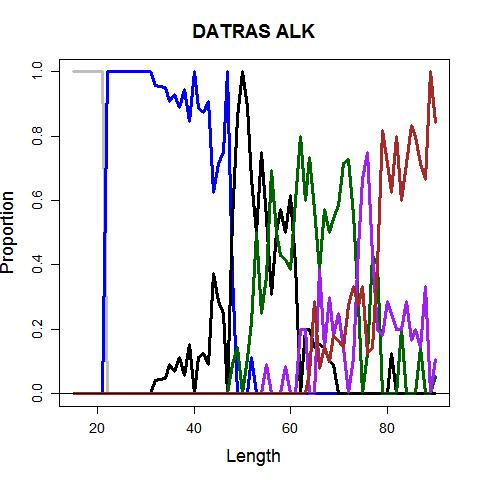
\includegraphics[scale=0.33]{figures/ALKdatrasQ1year2018RFA1.jpeg}}
\subfloat[]{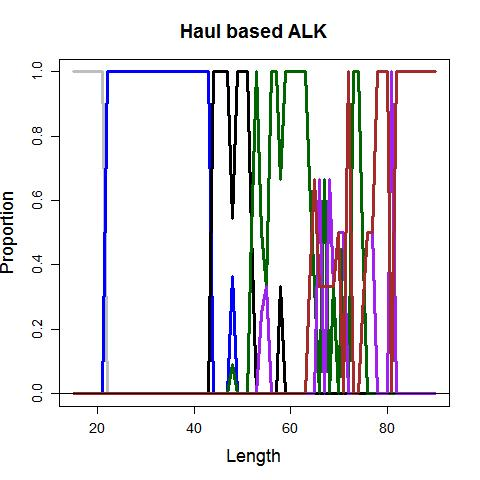
\includegraphics[scale=0.33]{figures/ALKhaulQ1year2018RFA1.jpeg}}
\subfloat[]{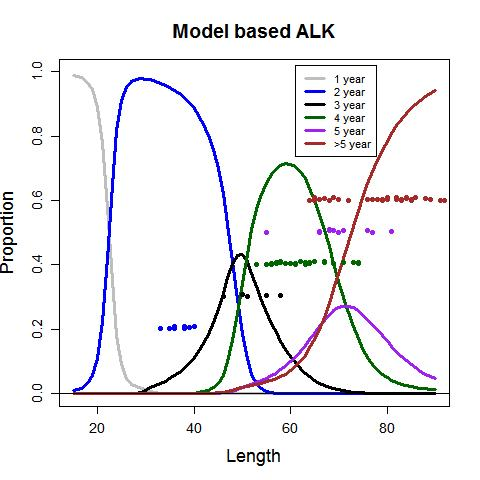
\includegraphics[scale=0.33]{figures/ALKmodelQ1year2018RFA1HaulWithMostObservations.jpeg}}
\captionsetup{font=small, width = 14.5cm}{
 \caption{Estimated age compositions of cod as a function of length in a given haul in RFA 1 using a) DATRAS ALK, b) haul based ALK and c) model based ALK. Note that explanation of the colours are only given in c). Each coloured point in c) defines an observed cod with the corresponding length and age in the haul. The haul selected is the haul with most observed ages of cod in 2018 Q1. }\label{fig:proportionRFA1CodQ1}}
\end{figure}

With regards to how many otoliths to sample per length group, the evidence is clear that .....\\

{\bf discuss DATRAS and Haul based ALK and recommended optimum sampling level of otoliths per length group}


%\begin{itemize}
%\item \citet{aanes2015efficient} suggested checks when using ALK for estimating relative abundance at age. Are any of these plausible things for us to consider, perhaps to address the issues with spatial ALK model base?
%\begin{enumerate}
%\item Check correlation between cluster size (catch weight/ number). If there is, weighting the age data by cluster size (number of fish per trawl haul) is advisable
%\item Check the sensitivity of various approaches e.g., length stratified, random, reduction/increase in sample size. If these are not possible, it might be useful to set up some experiments, e.g., surveys
%\item When borrowing ALK data from a different stratum (gear, quarter, area), check for differences in the age structure between the strata.
%\end{enumerate}
%\end{itemize}
%
%The optimum level sampling procedure employed showed that  

%Alternatively, one can apply the design base spatial ALK (haul base), which gave comparable estimates as the spatial ALK model. 
%Precision for relative abundance from the spatial model base estimator cannot be determined using the Fisher Information matrix because of  from the  is obtained by bootstrapping

%\begin{itemize}
%\item \emph{discuss positives of using GRT to model spatial effects: what problems are eliminated when using this in terms of missing data}
%\item \emph{compare the effects of our method with GAMs \citep{berg2012spatial} and \citep{berg2014evaluation} and the NS-IBTS Delta-GAM index for estimating standardized age-based indices and the species theses are used for to include in assessment}
%\item \emph{what does our model allows in terms of the age groups (samller or higher age groups (6+) possible with our model); covariates such as haul effect (included as a random effect)}
%\end{itemize}
%
%Also, both spatial ALK methods proposed in this paper provided a much better fit to the data compared with DATRAS ALK....
%
%Reducing the number of otoliths by ${\bf x}$ percent had {\bf no} significant effect on estimated abundance
%\begin{itemize}
%\item \emph{discuss sampling procedure: limitation and advantages; and possibly more advanced selection procedures? }
%\item \emph{new approach adopted in surveys from 2018 }
%\item \emph{IBTS has a standardized survey indices? -(yes Berg's NS-IBTS Delta-GAM index).  so changes in catch rates are due to changes in population size? \citet{berg2014evaluation} developed a standardized index for IBTS data but only applied to some species e.g., haddock? cod- last year 2017. Is the designed based age index on DATRAS not a standardized index?}
%\item \emph{how does changes in survey design or other factors affect changes in catch rates? If so are these changes  significant? }
%\end{itemize}

%
%\clearpage
%\section{General comments}
%
%\begin{itemize}
%\item Decide on whether we say, "in this research or paper"
%\item Decide on whether to say, "In this subsection or section"
%\item Decide on year of data for case studies
%\item Decide on writing "haul(model)-based or haul (model) based
%\item Decide on calling the survey "The North Sea IBTS or IBTS"
%\item Decide on writing "Cod or cod, and Saithe or saithe"
%\item Decide on a title for the paper
%\item {\bf what are issues with including haul effect in model based ALK?
% (Olav)}
% 
%\end{itemize}

\clearpage








\clearpage

\bibliographystyle{apalike}
\bibliography{ibtsBib}

\clearpage


\begin{center}
\textbf{\Large Supplemental Materials: Optimizing sampling effort of the North Sea International Bottom Trawl Survey.}
\end{center}
%%%%%%%%%% Merge with supplemental materials %%%%%%%%%%
%%%%%%%%%% Prefix a "S" to all equations, figures, tables and reset the counter %%%%%%%%%%
\setcounter{section}{0}
\setcounter{equation}{0}
\setcounter{figure}{0}
\setcounter{table}{0}
\setcounter{page}{1}
\makeatletter
\renewcommand{\thesection}{S\arabic{section}}
%\renewcommand{\theequation} {\arabic{section}. S\arabic{equation}}
%\renewcommand{\theequation}{S\arabic{equation}}
\renewcommand{\theequation}{S\arabic{section}.\arabic{equation}}
\renewcommand{\thefigure}{S\arabic{figure}}
\renewcommand{\bibnumfmt}[1]{[S#1]}
\renewcommand{\citenumfont}[1]{S#1}

\setcounter{table}{0}
\numberwithin{table}{section}
%\clearpage
\section{\large Areas fished by different countries in the North Sea IBTS}
\label{secAp:areasfishedappendix}
Typically, two different countries fish each rectangle so that at least two trawl hauls are made per rectangle, but intensified sampling is carried out in the following areas: at least 3 hauls per rectangle are taken in statistical rectangles  31F1, 31F2, 32F1, 33F4, 34F2, 34F3, 34F4, 35F3, 35F4; while six or more hauls per rectangle are taken in statistical rectangles  30F1, 32F2, 32F3, 33F2, 33F3 (ICES 1999).  The Skagerrak and Kattegat is fished solely by Sweden, who sample more than once in every rectangle while the west of Shetland (in Q1 and Q3) and inshore areas (Q3) is fished solely by Scotland. The edge of the Norwegian Trench is fished solely by Norway, but inshore areas near Denmark is fished by Denmark. The southern North Sea is fished by Denmark, Germany and England. France, typically, is the only country that surveys the western English Channel. Areas are surveyed by a single country because of the large proportion of untrawalable area (and subsequent gear damage issues experienced by other nations)  for efficient logistical purposes. Table \ref{countries} gives the countries and research vessels participating the North Sea IBTS.\\
\begin{small}
\begin{table}[h!]
\centering
\captionsetup{font=small, width = 15.5cm}{
\caption{Survey countries, vessel name, and period research vessels participating in first quarter (Q1) and third quarter (Q3) during 1997-2017.}\label{countries}}
\begin{tabular}{cccccccc}
\hline \\[0.1ex]
  & \multicolumn{2}{c}{\bf First Quarter (Q1)} & \multicolumn{2}{c}{\bf Third Quarter (Q3)}\\[1.5ex]
{\bf Country }  & Vessel name & Period    & Vessel name & Period  \\[0.5ex]
\hline \\[0.5ex]
Denmark  &   Dana   &   January-February  & Dana & July-August    \\[1ex]
France  & Thalassa II & January-February & - & -   \\[1ex]
Germany   &  Walther  Herwig III & January-February   &   Walther  Herwig III & July-August \\[1ex]
Netherlands &  Tridens 2 &  January-February   & - & -     \\[1ex]
Norway  &   G.O. Sars  & January-February &    Johan Hjort  & July   \\[1ex]
UK England &- & -&  Endeavour &  August-September  \\[1ex]
UK Scotland   &  Scotia III &  January-February & Scotia III &  July-August \\[1ex]
Sweden  &  Dana &  January-February  &  Dana &  August                  \\[0.5ex]
\hline
\end{tabular}
\end{table}
\end{small}

%\clearpage
\section{\large Otolith sampling per fish species}
\label{secAp:otolithappendix}
From 1991-2017, most countries conducted quota sampling of otoliths per length group in a RFA. But from 2013 Norway has been sampling one otolith per length class from each trawl haul (to 0.1$\cm$ below for shellfish, to 0.5$\cm$ below for herring and sprat and to 1$\cm$ below for all other species). From the first quarter in 2018 all countries are required to sample one otolith per length class per trawl haul.  Table \ref{tab:otolithsTable} gives the minimum sampling levels of otoliths for the target species. However, for the smallest size groups, that presumably contain only one age group, the number of otoliths per length class may be reduced, and more otoliths per length are required for the larger length classes. %\\
%\clearpage
\begin{small}
\begin{table}[h!]
\centering
\caption{Minimum sampling levels of otoliths by species for RFA or per trawl haul.}
\label{tab:otolithsTable}
\begin{tabularx}{\linewidth}{r l l l l X}
\toprule 
Period &  Species  & Minimum sampling levels of otoliths per length class    \\[0.7ex]
\midrule \\[0.1ex]
{\bf 1991-2017} & & {\bf Number of otoliths per length class in a RFA}  \\[1.0ex]
     & herring  &  $8$  otoliths per $\frac{1}{2}$ cm group \\[0.5ex]
     & sprat    & $16$  otoliths per $\frac{1}{2}$ cm length class  $8.0 -11.0$ cm\\[0.5ex]
              & & $12$  otoliths per $\frac{1}{2}$ cm length class  $\geq 11.0$ cm\\[0.5ex]
& mackerel      & $8$  otoliths per $\frac{1}{2}$ cm length class \\[0.5ex]
& cod       	  & $8$  otoliths per $1$ cm length class\\[0.5ex]
&haddock   	  & $8$  otoliths per $1$ cm length class \\[0.5ex]
&whiting    	  & $8$  otoliths per $1$ cm length class \\[0.5ex]
&Norway pout   & $8$  otoliths per $1$ cm length class\\[0.5ex]
&saithe        & $8$  otoliths per $1$ cm length class \\[1ex] 
& All target species      &  From 2013 Norway and Scotland, and  Netherlands from 2016 \\[0.7ex] 
&& have been sampling 1 otolith per length class from each trawl haul \\[0.7ex] 
&& (to 0.1$\cm$ below for shellfish, to 0.5$\cm$ below for herring and sprat, and \\ [0.7ex] 
&& to 1$\cm$ below for all other species).\\[1.7ex] 

{\bf 2018} & & {\bf Number of otoliths per length class per trawl haul}  \\[1.0ex]
  & herring  &  $1$  otolith per $\frac{1}{2}$ cm group \\[0.5ex]
     & sprat    & $1$  otolith per $\frac{1}{2}$ cm length class  $8.0 -11.0$ cm\\[0.5ex]
              & & $1$  otolith per $\frac{1}{2}$ cm length class  $\geq 11.0$ cm\\[0.5ex]
& mackerel      & $1$  otolith per $1$ cm length class \\[0.5ex]
& cod       	  & $1$  otolith per $1$ cm length class\\[0.5ex]
& haddock & $2$  otoliths per $5$ cm length class $11 -15, \ 16-20, \ 21-25, \ 26-30$ cm \\[0.5ex]
& Norway pout & $2$  otoliths per $5$ cm length class $5 -10, \ 11-15$ cm\\[0.5ex]
               & & $2$  otoliths per $1$ cm length class $> 15$ cm\\[1.0ex]
&saithe        & $1$  otolith per $1$ cm length class \\[0.5ex]  
&plaice       & $1$  otolith per $1$ cm length class \\[0.1ex]
\bottomrule         
\end{tabularx}
\end{table}
\end{small}

%\clearpage
 \section{\large Weightings of Statistical Rectangles}
 \label{secAp:weightings}
 
 The weightings of the some statistical rectangles are alloted to species such as sprat, saithe and herring by depth strata. Table \ref{tab:weights} gives these weights, which are used in the analysis of the saithe data.\\
 
%\clearpage 
 \begin{small}
\begin{table}[h!]
\centering
\caption{Weights used for Pollachius virens in equation (\ref{eq:cpueRec}).}
\begin{footnotesize}
\begin{tabular}{clclclclcl}
  \hline \\ [0.3ex]
 StatRec & Weight & StatRec & Weight & StatRec & Weight & StatRec & Weight & StatRec & Weight  \\ [1.0ex]
  \hline \\ [0.3ex]
 31F1 &  0.6 & 38F0 &    1 & 41F7 &    1 & 44F3 &    1 & 48E7 &    1 \\ 
 31F2 &  0.8 & 38F1 &    1 & 41F8 &  0.1 & 44F4 &    1 & 48E8 &  0.9 \\ 
 31F3 & 0.05 & 38F2 &    1 & 41G0 &  0.2 & 44F5 &  0.9 & 48E9 &    1 \\ 
 32F1 &  0.8 & 38F3 &    1 & 41G1 & 0.97 & 44F8 & 0.25 & 48F0 &    1 \\ 
 32F2 &    1 & 38F4 &    1 & 41G2 & 0.53 & 44F9 &  0.8 & 48F1 &    1 \\ 
 32F3 &  0.8 & 38F5 &    1 & 42E7 &  0.4 & 44G0 & 0.94 & 48F2 &    1 \\ 
 32F4 & 0.01 & 38F6 &    1 & 42E8 &    1 & 44G1 &  0.6 & 48F3 &  0.5 \\ 
 33F1 &  0.3 & 38F7 &    1 & 42E9 &    1 & 45E6 &  0.4 & 48G0 & 0.02 \\ 
 33F2 &    1 & 38F8 &  0.3 & 42F0 &    1 & 45E7 &    1 & 49E6 &  0.8 \\ 
 33F3 &    1 & 39E8 &  0.5 & 42F1 &    1 & 45E8 &    1 & 49E7 &    1 \\ 
 33F4 &  0.4 & 39E9 &    1 & 42F2 &    1 & 45E9 &    1 & 49E8 &  0.4 \\ 
 34F1 &  0.4 & 39F0 &    1 & 42F3 &    1 & 45F0 &    1 & 49E9 &    1 \\ 
 34F2 &    1 & 39F1 &    1 & 42F4 &    1 & 45F1 &    1 & 49F0 &    1 \\ 
 34F3 &    1 & 39F2 &    1 & 42F5 &    1 & 45F2 &    1 & 49F1 &    1 \\ 
 34F4 &  0.6 & 39F3 &    1 & 42F6 &    1 & 45F3 &    1 & 49F2 &    1 \\ 
 35F0 &  0.8 & 39F4 &    1 & 42F7 &    1 & 45F4 &  0.6 & 49F3 &  0.5 \\ 
 35F1 &    1 & 39F5 &    1 & 42F8 &  0.2 & 45F8 &  0.3 & 50E6 &  0.1 \\ 
 35F2 &    1 & 39F6 &    1 & 42G0 & 0.32 & 45F9 & 0.02 & 50E7 &  0.6 \\ 
 35F3 &    1 & 39F7 &    1 & 42G1 & 0.89 & 45G0 & 0.24 & 50E8 &  0.7 \\ 
 35F4 &  0.9 & 39F8 &  0.4 & 42G2 & 0.64 & 45G1 & 0.55 & 50E9 &  0.9 \\ 
 35F5 &  0.1 & 40E7 & 0.04 & 43E7 & 0.03 & 46E6 &  0.4 & 50F0 &    1 \\ 
 36F0 &  0.9 & 40E8 &  0.8 & 43E8 &  0.9 & 46E7 &  0.9 & 50F1 &    1 \\ 
 36F1 &    1 & 40E9 &    1 & 43E9 &    1 & 46E8 &    1 & 50F2 &    1 \\ 
 36F2 &    1 & 40F0 &    1 & 43F0 &    1 & 46E9 &    1 & 50F3 &  0.2 \\ 
 36F3 &    1 & 40F1 &    1 & 43F1 &    1 & 46F0 &    1 & 51E6 &    0 \\ 
 36F4 &    1 & 40F2 &    1 & 43F2 &    1 & 46F1 &    1 & 51E7 &    0 \\ 
 36F5 &    1 & 40F3 &    1 & 43F3 &    1 & 46F2 &    1 & 51E8 &  0.5 \\ 
 36F6 &  0.9 & 40F4 &    1 & 43F4 &    1 & 46F3 &  0.8 & 51E9 &    1 \\ 
 36F7 &  0.4 & 40F5 &    1 & 43F5 &    1 & 46F9 &  0.3 & 51F0 &    1 \\ 
 36F8 &  0.5 & 40F6 &    1 & 43F6 &    1 & 46G0 & 0.52 & 51F1 &    1 \\ 
 37E9 &  0.2 & 40F7 &    1 & 43F7 &    1 & 46G1 &  0.2 & 51F2 &  0.5 \\ 
 37F0 &    1 & 40F8 &  0.1 & 43F8 & 0.94 & 47E6 &  0.8 & 51F3 &    0 \\ 
 37F1 &    1 & 41E6 & 0.03 & 43F9 & 0.41 & 47E7 &  0.6 & 52E6 &    0 \\ 
 37F2 &    1 & 41E7 &  0.8 & 43G0 & 0.21 & 47E8 &    1 & 52E7 &    0 \\ 
 37F3 &    1 & 41E8 &    1 & 43G1 &  0.7 & 47E9 &    1 & 52E8 &    0 \\ 
 37F4 &    1 & 41E9 &    1 & 43G2 &  0.3 & 47F0 &    1 & 52E9 &  0.1 \\ 
 37F5 &    1 & 41F0 &    1 & 44E6 &  0.5 & 47F1 &    1 & 52F0 &  0.2 \\ 
 37F6 &    1 & 41F1 &    1 & 44E7 &  0.5 & 47F2 &    1 & 52F1 &  0.5 \\ 
 37F7 &    1 & 41F2 &    1 & 44E8 &  0.9 & 47F3 &  0.6 & 52F2 &  0.1 \\ 
 37F8 &  0.8 & 41F3 &    1 & 44E9 &    1 & 47F9 & 0.01 &  &  \\ 
 38E8 &  0.2 & 41F4 &    1 & 44F0 &    1 & 47G0 &  0.3 &  &  \\ 
 38E9 &  0.9 & 41F5 &    1 & 44F1 &    1 & 47G1 & 0.02 &  &  \\ 
 52F3 &    0 & 41F6 &    1 & 44F2 &    1 & 48E6 &    1 &  &  \\ 
   \hline \\[0.8ex]
\end{tabular}
\label{tab:weights}
\end{footnotesize}
\end{table}
 \end{small}
 
% \clearpage
\section{\large Imputation for missing age samples}
\label{sec:imputationappendix}
Catches of the target species are sampled (or subsampled with a size of 100 if the catches are too large) for length, and otoliths are typically collected from a subsample of the individuals sampled for length in the RFA,  or per trawl haul as in the case of Norway for determining age of the fish (see Table \ref{otolithsTable}). In the case of Norway where all trawl hauls are sampled for otoliths, missing age samples would still occur for the following two reasons: 1) the fish is below minimum length for otolith sampling (unreadable otoliths) or 2) otoliths are misplaced. Abundance indices by age group are estimated based on three age-length-keys (ALK): 1) DATRAS ALK estimator, 2) Haul based ALK estimator, and 3) Spatial model based ALK estimator.
\subsection{\normalsize DATRAS ALK Borrowing Approach}
\label{secAp:DATRASBorrow}
The ALK proposed in DATRAS (ICES 2013), which is an aggregation of individual samples from a haul combined over a round fish area (RFA), and missing age samples are imputed as follows: 
\begin{enumerate}
\item If there is no ALK for a length in the CPUE dataframe, age information is obtained accordingly
\begin{itemize}
\item If length class (CPUE) $<$ minimum length class (ALK), then age=1 for the first quarter and age=0 for all other quarters
\item  If minimum length class (ALK) $<$ length class (CPUE) $<$ maximum length (ALK) then age is set to the nearest ALK. If the ALK file contains values at equal distance, a mean is taken from both values. 
\end{itemize}
\item If length class (CPUE) $>$ maximum length (ALK) age is set to the plus group.
\end{enumerate}
The underlying assumption of this ALK approach is that age-length compositions are homogeneous within the RFA. 
\subsection{\normalsize Haul based ALK Borrowing Approach}
\label{secAp:oursBorrow}
\indent  The second is an a haul dependent ALK estimator which we propose, and is denoted by $\mathrm{ALK}^{H}$. Since the age-length composition of fish may be space-variant, that is, there may be variation in age-length compositions between trawl stations within a RFA, the spatial dependence of the age-length composition must be accounted for to produce reliable estimates of the CPUE per age estimates. If this spatial dependence is ignored not only will estimates of abundance be biased but the impact on the variance may be substantial. So for each trawl haul an $\mathrm{ALK}^{H}$ is produced. To replace missing values for the age distribution in a length class the method of "borrowing" ages from the same length  from neighbouring trawl hauls of maximum radius of two statistical rectangles within the RFA. If there are no observed ages in the length class from the neighbour hauls in the RFA, missing values for the age distribution are replaced following the procedure outlined in the DATRAS ALK procedure (\ref{secAp:DATRASBorrow}) in step 1. 


%{\bf Since there are few or none observations of ages for each length class in a trawl haul, length classes are therefore pooled in increasing order such that there are five length classes in each pooled length group. To replace missing values for the age distribution in the pooled length groups the method of "borrowing" ages from length groups in trawl hauls closest in air distance within the RFA is used. If there are no observed ages in the pooled length group in the RFA, missing values for the age distribution are replaced following the procedure outlined in the DATRAS ALK procedure (\ref{secAp:DATRASBorrow}) in step 1.  }

\section{\large Nonparametric Bootstrap Sampling procedure}
\label{secAP:nonparametricbootstrap}
Nonparametric bootstrapping is attractive as it makes no distributional assumption, and is suitable for estimating confidence interval for indices of abundance. Suppose we have a vector $\bf x$ of $m$ independent observations, and we are interested in estimating a parameter $\hat{\theta} ({\bf x})$ and its variance. The general nonparametric bootstrap algorithm is as follows:
\begin{enumerate}
\item Sample $m$ observations randomly with replacement from ${\bf x}$ to obtain a bootstrap data set, denoted by ${\bf {x}^{*}}$.
\item Calculate the bootstrap version of the statistic of interest, ${\theta}^{*} = \hat{\theta}({\bf {x}^{*}})$.
\item Repeat steps 1 and 2 a large number of times, say $B$, to obtain an estimate of the bootstrap distribution
\item calculate the average of the bootstrapped statistics, $\sum_{b=1}^{B} {{\theta}^{*}}_{(b)}/B$ 
\item compute the variance of the estimator $\hat{\theta}({\bf x})$ through the variance of the set ${{\theta}^{*}}_{(b)}, \ b = 1,2,...,B,$ given by 
\begin{equation}
\frac{ \sum_{b=1}^{B} {\left({{\theta}^{*}}_{(b)} - {{\theta}^{*}}_{(\cdot)} \right)}^{2}  }{(B-1)} 
\end{equation}
where ${{\theta}^{*}}_{(\cdot)} = \sum_{b=1}^{B} {{\theta}^{*}}_{(b)}/B. $
\end{enumerate}
The Bias-Corrected method assumes that there is a montonic increasing function and the estimator $\hat{\lambda}_{a}$ has a monotonic increasing function $f()$ such that the transformed values $f(\hat{\lambda}_{a})$ are normally distributed with mean $f(\lambda_{a}) - z_{0}$ and standard deviation one, where $z_{0}$ are the standard normal limits \citep{puth2015variety, karlsson2009bootstrap}. Now, let $P^{*} \left(\hat{\theta} ({\bf x^{*}}) \leq \hat{\theta} ({\bf x}) \right) $ denote the proportion of $\hat{\theta} {({\bf x^{*}})}^{'} \mathrm{s}$ in the bootstrap sample that have a value lower than the value of the parameter estimate $\hat{\theta} ({\bf x})$, and le $z_{0}$ be defined as
\begin{equation}
 z_{0} = \Phi^{-1} \left\{ P^{*} \left(\hat{\theta} ({\bf x^{*}}) \leq \hat{\theta} ({\bf x}) \right) \right\}, 
\end{equation}
\noindent where $  \Phi $  denotes the cumulative distribution function of the standard normal distribution. Also let $\tilde{\alpha}_{1} $ and $\tilde{\alpha}_{2} $ be defined as
\begin{equation}
\tilde{\alpha}_{1} = \Phi(2z_{0} + z_{\alpha}), 
\end{equation}
\noindent and 
\begin{equation}
\tilde{\alpha}_{2} = \Phi(2z_{0} + z_{1-\alpha}), 
\end{equation}
\noindent respectively.  A $100(1-2 \alpha)$ percent confidence interval for $ \theta ({\bf x})$ is then given by
\begin{equation}
\hat{\theta}_{\left(\tilde{\alpha}_{1}(B +1) \right)} ({\bf {x}^{*}})  \leq \hat{\theta} ({\bf x}) \leq \hat{\theta}_{\left((\tilde{\alpha}_{2} -1)(B +1) \right)} ({\bf {x}^{*}}). 
\end{equation}

\section{\large IBTS data set for cod and saithe}
\label{secAp:data}
%\clearpage
\begin{small}
\begin{table}[h!]
\caption{Summary of North Sea IBTS cod and saithe (in parentheses) data for third quarter in year 2017 and first quarter in year 2018.}
\begin{tabular}{llllll}
\toprule
\bf Data&\bf Description \\
\midrule
Trawl hauls  & Total of 372 trawl hauls in year 2018 Q1; 238 (83)  with length and 230 (81) \\ & with age information. In 2017 Q3, a total of 345  trawl hauls were taken; \\ & 238 (129) with length and 237 (128) with age information. \\[1.7ex]

Age &The age varied between 1 (1) to 12 (18) years in year 2018 Q1 and \\ & 0 (0) to 11 (17) in year 2017 Q3. \\[1.7ex]

Length & Length information in cm varied between 11 (13) to 114 (106) cm in year 2018 Q1 \\ & and between 6 (10) to 112 (109) cm in year 2017 Q3. \\[1.7ex]

Date&Date of catch in year 2018 Q1 varied between 15.01.2018 to 28.02.2018 \\ & and in year 2017 Q3 between 18.07.2017 to 31.08.2018 \\[1.7ex]

Duration of haul & Mean duration is 29.37 minutes, with 30 minutes as 83\% coverage interval \\ & in year 2018 Q1; and in 2017 Q3 with mean duration of 29.26 minutes \\ & with 30 minutes as 88\% coverage . \\[1.0ex]

Total count for all ages & 1600 (822) in year 2018 Q1 and 2330 (2163) 2017 Q3. \\[0.5ex]
\bottomrule
\end{tabular}
\label{tab:data2018}
\end{table}
\end{small}


 \begin{small}
\begin{table}[h!]
\centering
\caption{Age and length data for saithe in year 2017 Q3 and cod in year 2018 Q1. Data collected in the first quarter (Q1) has no age 0 group but this is collected in quarter 3 (Q3) surveys.}
\begin{footnotesize}
\begin{tabular}{clclclclclclclclclclclclclclclclclclclclclclclclclclclclclclclclclcl}
  \hline \\ [0.3ex]
  & \multicolumn{6}{c}{\bf saithe in year 2017 Q3} &   \multicolumn{6}{c}{\bf cod in year 2018 Q1} \\[2.0ex]
  \cmidrule(lr{0.3em}){2-7}  \cmidrule(lr{0.3em}){8-13}  \\ [0.5ex]
 Age & \thead{Numbers \\ aged} & $\bf L_{min}$ & $\bf L_{max}$ & $\bf L_{mean}$ & Sd($\bf L$) & CV($\bf L$) & \thead{Numbers \\ aged} & $\bf L_{min}$ & $\bf L_{max}$ & $\bf L_{mean}$ & Sd($\bf L$) & CV($\bf L$) \\ [1.0ex]
 % \hline \\ [0.3ex]
  \cmidrule(lr{0.3em}){2-7}  \cmidrule(lr{0.3em}){8-13}  \\ [0.5ex]
 0 &  21 & 10   & 14 & 12.143 & 1.195 &  0.098   &      &      &      &     \\ [1.5ex]
 1 &  26 & 23   & 32 & 27.654 & 2.297 &  0.083   & 149  &  11  & 30   &  18.407 & 3.693  & 0.201 \\ [1.5ex]
 2 &  65 & 27   & 47 & 38.077 & 3.337 &  0.088   & 814  &  17  & 53   &  33.180 & 6.290  & 0.190  \\[1.5ex] 
 3 & 531 & 34   & 56 & 42.041 & 3.785 &  0.090   & 222  &  30  & 81   &  50.654 & 10.185 & 0.202 \\ [1.5ex]
 4 & 767 & 35   & 73 & 48.261 & 4.521 &  0.094   & 189  &  43  & 92   &  64.479 & 8.399  & 0.130  \\ [1.5ex]
 5 & 334 & 46   & 78 & 56.876 & 6.105 &  0.107   & 102  &  54  & 96   &  76.627 & 9.594  & 0.125 \\[1.5ex] 
 6 & 159 & 50   & 91 & 66.025 & 7.137 &  0.108   & 84   &  54  & 100  &  80.871 & 9.456  & 0.117 \\[1.5ex] 
 7 & 127 & 57   & 93 & 73.976 & 7.163 &  0.097   & 28   &  58  & 110  &  84.086 & 11.308 & 0.134  \\[1.5ex] 
 8 & 69  & 63   & 94 & 77.725 & 7.010 &  0.090   & 4    &  80  &  94  &  85.500 & 6.455  & 0.075 \\ [1.5ex]
 9 & 18  & 64   & 97 & 85.333 & 7.499 &  0.088   & 5    &  66  &  96  &  83.400 & 11.305 & 0.061 \\ [1.5ex]
10 & 22  & 84   &107 & 92.364 & 5.803 &  0.063   & 1    &  87  &  87  &  -      & -      & -   \\ [1.5ex]
11 &  5  & 79   &102 & 92.800 & 9.311 &  0.100   & 1    & 106  & 106  &  -      & -      & -   \\ [1.5ex]
12 &  7  & 91   &109 & 99.429 & 6.554 &  0.066   &      &      &     \\ [1.5ex]
13 &  5  & 94   &104 & 98.800 & 4.550 &  0.046   &      &      &     \\ [1.5ex]
14 &  1  & 108  &108 & 108    & -     &  -       &      &      &     \\ [1.5ex]
15 &  1  & 105  &105 & 108    & -     &  -       &      &      &     \\[1.5ex] 
16 &  4  & 93   &106 & 100.250& 5.439 &  0.054   &      &      &   \\ [1.5ex]
17 &  1  & 109  &109 & 109    & -     &  -       &      &      &   \\ [0.5ex]
 
   \hline \\[0.8ex]
\end{tabular}
\label{realdatacodandsaithe}
\end{footnotesize}
\end{table}
 \end{small}
 

\section{\large Estimates from DATRAS and Stratified bootstrap procedures}
\label{secAp:resultsdatrasALK}
The bootstrap procedure proposed by DATRAS lacks the potential to account for the spatial variation in the data. The DATRAS bootstrap procedure ignores the fine-scale stratification in the sampling process, leading to an overestimation of the uncertainty; and ignores the age-length data collected at the haul level, resulting in an underestimation of the uncertainty. The results (Figure\ref{DatrasStratified}) shows an overestimation of the uncertainty for all age groups, suggesting that it is relevant to account for the fine-scale stratification when resampling the data.

\clearpage
\begin{figure*}[h!]
\centering
\begin{tabular}{@{}ccc@{}}
\subfloat[Datras and Stratified bootstrap Procedures]{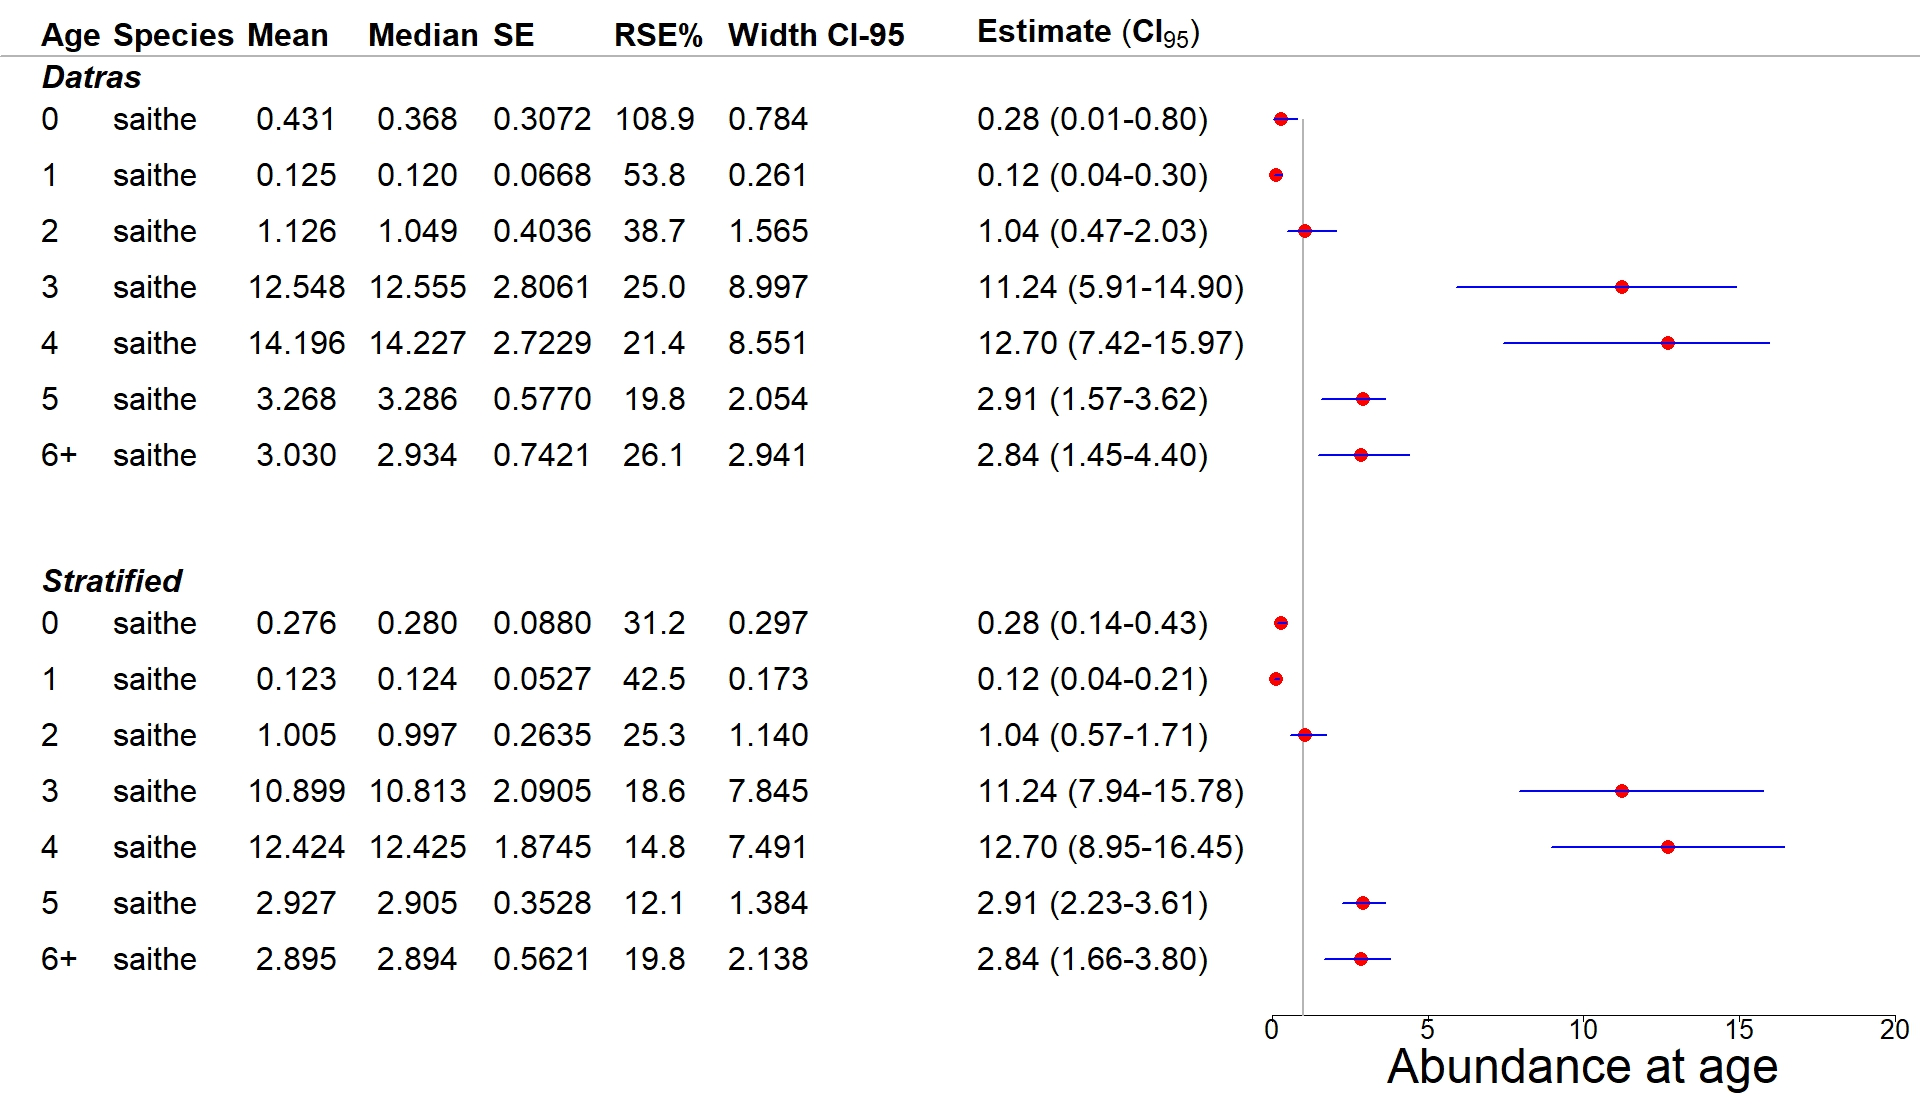
\includegraphics[width=0.95\textwidth]{figures/saithe2017Q3DATRASStratifedBiasCorr.jpeg}} & 
\end{tabular}
\caption[]{Comparison of estimated confidence intervals ($\mathrm{CI}_{95}$) from DATRAS and stratified bootstrap procedures. The bias-corrected bootstrap method is used to give estimates for saithe in year 2017 Q3. Estimated indices of abundance (Estimate), and its standard error (SE), bootstrap mean (Mean), Median estimates, percentage relative standard error (RSE \%) and width of confidence intervals  are also given.}
\label{DatrasStratified}
\end{figure*} 


\end{document}